%\documentclass[prd, nofootinbib, floatfix, 12pt]{revtex4}
%\documentclass[useAMS,usenatbib,11pt,preprint]{aastex}
%\documentclass[12pt,preprint]{aastex}
\documentclass[11pt]{article}
\usepackage{amsmath}
\usepackage{amsbsy}
\usepackage{natbib}
\usepackage{graphicx}

\usepackage[paperwidth=8.5in,paperheight=11in,centering,hmargin=1in,vmargin=1in]{geometry}
%\usepackage[round]{natbib}
%\usepackage{float}
%\usepackage{amsmath}
%\usepackage{amsbsy}
\usepackage{caption}
\usepackage{subcaption}

\topmargin0.0cm
\textheight8.5in

%\input epsf
%\usepackage{amsmath,amssymb}
%\usepackage[margin=0in]{caption}
%\usepackage{subfigure}
%\usepackage{epsfig}
%\usepackage{color}
%\usepackage{ulem}
%\usepackage{epstopdf}

\renewcommand{\topfraction}{0.95}
\renewcommand{\bottomfraction}{0.95}


%%%%%%%%%%%%%%%%%%%%%%%%%%%%%%%%%%%%%%%%%%%%%%%%%%%%%%%%%%%%
%%%%%%%%%%%%%%%%%%%%%%%%%%%%%%%%%%%%%%%%%%%%%%%%%%%%%%%%%%%%
%%%%%%%%%%%%%%%%%%%%%%%%%%%%%%%%%%%%%%%%%%%%%%%%%%%%%%%%%%%%

\begin{document} 

\captionsetup{width=0.87\textwidth}

\title{The LSST Universe model and its validation}

\author{ Simon Krughoff, Andrew Connolly, Yusra AlSayyad, Lynne Jones, Rob Gibson,
  Mario Juri{\'c}, {\V Z}eljko, Debbie Bard, for the LSST Collaboration}

%\pagerange{\pageref{firstpage}--\pageref{lastpage}}

\label{firstpage}

\date{\today}

\maketitle 


\abstract{The Large Synoptic Survey Telescope (LSST) will produce a
  wide-field and multi-epoch imaging survey of 18,000 deg$^2$ of the
  southern sky.  The LSST has an 8.4m aperture (with an effective size
  of 6.7m) and a 9.6 deg$^{2}$ field of view.  The large etendue of
  the LSST enables the project to image the visible sky every 3
  nights. To evaluate the performance of the LSST, to design the
  algorithms used in processing the LSST data, and to enable the
  development of science analysis techniques in preparation for
  operations, the LSST has undertaken a program for high fidelity
  simulations.  These simulations include a realistic model of the
  universe (known as the base catalog or universe model), a framework
  for querying the model at specific points on the sky and instances
  in time (known as the catalog framework), and a fast ray-trace code for
  simulating raw images (PhoSim).  In this document we describe the
  base catalogs and catalogs framework (known together as CatSim) and
  validate them for use by the LSST project.  The requirements against
  which we will validate are described in the document ``Requirements
  for the LSST Simulation Framework''. }
 
\section{Introduction \label{sec:intro}}

A new generation of astronomical survey telescopes such as the Large
Synoptic Survey Telescope (LSST) will soon be surveying the universe
in unprecedented detail. Repeated observations of the same part of the
sky, with hundreds to thousands of observations over a period of ten
years, will enable detailed studies of the temporal universe (ranging
from transient sources such as supernovae and optical bursters, to
periodic variables such as Cepheids and RR-Lyrae stars, to moving
sources such as asteroids and high proper motion stars). Combination
of these observations will provide some of the deepest, large-scale
surveys of the universe ever undertaken and provide the ability to
measure the nature of dark energy with figures of merit 10-100 times
smaller than current surveys \citep[DETF][]{albrecht06}.

The stringent requirements on the statistical power of the LSST means
that we will soon no longer be limited by shot noise (i.e.\ the number
of sources within a sample) but by how well we can understand
systematic uncertainties within our data streams. These systematic
effects can arise from the design of the telescope (e.g.\ ghosting of
images or scatter light), from the response of the atmosphere (e.g.\
the stability of the point-spread-function or the variability in the
transmissivity of the sky), from the strategy used to survey the sky
(e.g.\ inhomogeneous sampling of astronomical light curves), or from
limitations in our analysis algorithms (e.g.\ due to the finite
processing power available approximations may need to be made when
characterizing the properties of detected sources). Understanding
which of these issues will impact the science from a given telescope
is imperative if we hope to maximize their scientific returns.

Simulations of the data flow from survey telescopes can provide a
critical role in understanding the capabilities of an astronomical
system and in optimizing its scientific returns. By providing data
with the expected characteristics of a survey well in advance of first
light, algorithms and statistical techniques can be optimized and
scaled to the expected data volumes or new statistical approaches can
be developed to improve the data analysis.  In the following sections
we consider and describe how we model the astrophysical properties of
the universe that we expect the LSST to observe and validate the
properties of this model universe against the requirements of the
project \citep{requirements}.

\section{Source Catalogs and the Catalog Framework}

\subsection{Framework}

The design of a framework to simulate the data expected from the LSST
requires flexibility and scalability \citep{connolly10}.
%(to enable
%data generation runs that range from a single CCD image of a
%gravitational lens to images from thousands of full focal planes that
%trace the expected observing cadence of the survey). 
This is accomplished by dividing the simulation workload into three
separate components: a base component that stores a model of the
universe (including the distribution of galaxies from a cosmological
simulation, the distribution of stars from a Galactic Structure model,
and a model for the asteroid populations within our Solar System), a
system for querying the underlying model of the universe using
simulations of sequences of LSST observations, and a framework for the
generation of images via the ray-tracing of photons from individual
sources.

Figure~\ref{fig:flow} shows the flow of information through the LSST
simulation framework.
%Simulations of sequences of
%LSST observations enable catalogs of LSST sources to be
%generated. These catalogs can be analyzed for different science
%programs or passed to a photon based image generator that create input
%images for the data management analysis pipelines.  
This design enables the generation of a wide range of data products:
from all-sky catalogs used in modeling the LSST calibration pipeline,
to time domain data used to characterize variability as a function of
signal-to-noise and temporal sampling, to sequences of images of
gravitational lenses from which to measure cosmological time delays.
In this document we focus on the first component of the framework; the
LSST universe model or base catalog and how we can query this
model. This system is referred to as {\it CatSim} throughout this
document.

The base catalog is stored as a SQL database (using a Microsoft
SQLServer). Data are accessed through a Python interface that uses
SQLalchemy ({\tt http://ls.st/f7e}) to provide a database
agnostic view of the sources. For LSST pointing, sources can be
queried as a function of position and time with the returned data
accounting for any change in brightness due to variability. For large
scale runs, the base catalog is queried using sequences of
observations derived from the Operations Simulator \citep{cook09} (see
also: {\tt http://ls.st/bta}).  The Operation Simulator
simulates LSST pointings that meet the cadence and depth requirements
of the LSST science cases while accounting for historical weather
patterns for Cerro Pach\'{o}n and the visibility of the LSST footprint on
the sky. Each simulated pointing provides a position and time of the
observation together with the appropriate sky conditions (e.g. seeing,
moon phase and angle, and sky brightness). Positions of sources are
propagated to the time of observation (including the proper motion
information for stars and orbits for Solar System sources). Magnitudes
and source counts are derived using the atmospheric and filter
response functions appropriate for the airmass of the observation and
after applying corrections for source variability. The resulting
catalogs (instance catalogs) can be formatted for use in a science
application (e.g. measuring the proper motions of high velocity stars)
or fed to the final component of the simulation framework, the image
simulator \citep{phosim}.

The query framework is written in Python and takes an object-centric
view of the data.  For each object type (galaxy, main sequence star,
strong lens, etc.), a class is defined that knows how to query for,
format, and transform objects of that type.  Many objects are similar
in terms of their properties and how they need to be queried.  A small
number of base classes can, therefore, be defined that will encompass
the requirements of the majority of the object classes.  Additional
object types are then represented simply as subclasses of the base
class. Extensibility of catalog types is handled by a class called the
InstanceCatalog, which defines how the output from the object classes
is formatted and written out into a catalogs.  Again, each catalog
type is a subclass of the base InstanceCatalog class, so extending to
other catalog types simply requires overriding the default formatter.
This also allows for custom headers (like those needed for input to
PhoSim) and custom output (e.g. binary, fits, or Python pickle files).

Overall this approach provides a simple and extensible framework for
expressing different astrophysical sources and incorporating new
catalogs within an existing framework (i.e.\ different components of
the universe model are logically distinct and so can be separated into
independent tables in a database or in different databases all
together).

\begin{figure}[h]
\centerline{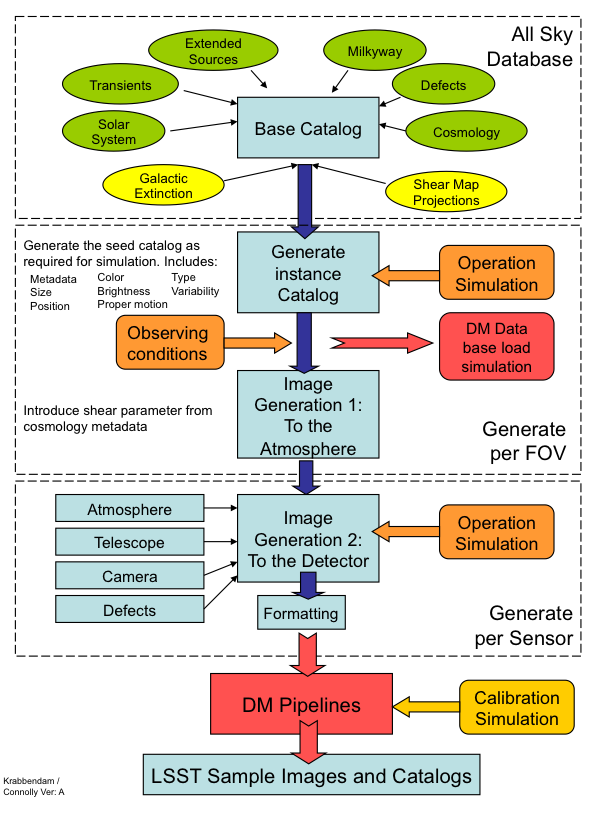
\includegraphics[width=0.5\textwidth]{validation_figures/flow.png}}
\caption{The flow of information through the LSST simulation
 framework. Databases of astrophysical sources are populated with
 models of the cosmological distributions of galaxies, the
 distributions of stars within our Galaxy, and the populations of
 asteroids within our Solar System. Using historical records for the
 weather at Cerro Pach\'{o}n and the observing cadences required by the
 science drivers for the LSST, sequences of simulated observations
 are generated by the Operations simulator. From these simulated
 pointings, catalogs and images of galaxies can be generated that
 match the expected properties of the LSST system. Comparing the
 catalogs derived by processing the LSST data with those used to
 generate the inputs we enable a full end-to-end test of the LSST
 system.}
\label{fig:flow}       % Give a unique label
\end{figure}


\subsection{Galaxies and Cosmology \label{sec:gal}}

The galaxy simulation is based on dark matter haloes from the
Millennium simulation \citep{springel05} (with an assumed standard
$\Lambda$-CDM cosmology) and a semi-analytic baryon model grafted upon
the Millennium results as described in \citet{springel05} and
\citet{delucia}. This semi-analytic model features radiative cooling,
star formation, and the dynamics of black holes, supernovae, and
AGNs. It includes explicitly following dark matter haloes, even after
accretion onto larger systems, in order to follow the dynamics of
satellite galaxies for an extended period of time as well as `radio
mode' feedback of AGNs. The model was adjusted to mimic the
luminosity, color, and morphology distributions of low redshift
galaxies \citep{delucia}. LSST cosmological catalogs were generated
from the \citet{delucia} data by constructing a lightcone, covering
redshifts 0$<$z$<$6, from 58 500h$^{-1}$Mpc simulation snapshots. This
lightcone covers a 4.5x4.5 degree footprint on the sky and samples
halo masses over the range $2.5\times10^9$ to $10^{12}$ $M_\odot$.

Dynamically tiling this footprint across the sky enables the
simulation of the full LSST footprint while keeping the underlying
data volume small (but at the expense of introducing periodicity in
the large scale structure).  For all sources, a spectral energy
distribution (SED), is fit to the galaxy colors using Bruzual and
Charlot spectral synthesis models \citep{bruzual}. The \citet{delucia}
catalog includes BVRIK magnitudes and dust values for the disk and
bulge components of each galaxy as well as radii, redshift,
coordinates, stellar age, masses and metallicities. These parameters
are used in constraining the assignment of SEDs to each disk and bulge
component.  Fits are undertaken independently for the bulge and disk
and include inclination dependent reddening. Morphologies are modeled
using two Sersi{\'c} profiles and a single point source (for the AGN)
with bulge-to-disk ratios and disk scale lengths from \citet{delucia}.
Half-light radii for bulges are estimated using the empirical
absolute-magnitude vs half-light radius relation given by
\citet{gonzalez09}.  AGNs are derived using the \citet{bongiorno12}
luminosity function. The B-band absolute magnitudes are converted to
bolometric luminosities using Eqn. 2 in \citet{hopkins07}. Empirical
relations derived from the SDSS enable computation of the colors and
stellar mass of the AGNs host galaxy from its luminosity. These
parameters are used, together with the redshift values from the AGN
catalog, to match each AGN to a galaxy in the galaxy catalog. In
general, the AGNs match to galaxies having higher stellar masses,
approximately $10^{9}$ to $10^{11}$ $M_{\odot}$ which is comparable to
recent analysis of host galaxies done by \citet{xue11}. The AGN SED is
taken from the mean AGN spectrum of \citet{vandenberk}.

Comparisons between the redshift and
number-magnitude distributions of the simulated catalogs with those
derived from deep imaging and spectroscopic surveys showed that the De
Lucia models under-predict the density of sources at faint magnitudes
and high redshifts. To correct for these effects, sources are
``cloned'' in magnitude and redshift space until their densities
reflect the average observed properties (see \S
\ref{sec:galaxycounts}).



\subsection{Galactic Structure \label{sec:stars}}

Stars are represented as point sources and are drawn from the Galfast
model of \citet{galfast}.  Galfast generates stars according to
density laws derived from fitting SDSS data to a model of a thick and
thin disk, and a halo \citep{juric}. Using an input luminosity
function measured from SDSS for each class of star (e.g.\ main
sequence, white dwarf, blue horizontal branch, etc.), Galfast samples
stars in space and magnitude from a 4-dimensional probability density
function $\rho$(x,y,z,M). After this stage, using Fe/H and kinematics
models from \citet{ivezic08} and \citet{bond09} (also derived from
SDSS data), each star is assigned a metallicity, proper motion, and
parallax.  Spectral energy distributions are fit to the predicted
colors using the models of \citet{kuruczCD} for main sequence stars
and giants, \citet{bergeron95} for white dwarfs, and a combination of
spectral models and SDSS spectra for M, L, and T dwarfs
\citep[e.g.][]{cushing05,bochanski07,burrows06,pettersen89,kowalski10}.
For Galactic reddening, a value of E(B-V) is assigned to each star
using the three-dimensional Galactic model of \citet{amores05}. For
consistency with extragalactic observations the dust model in the
Milky Way is re-normalized to match the \citet{schlegel98} dust maps
at a fiducial distance of 100 kpc.  Once the extinction and SED are
assigned, observed magnitudes are calculated in the SDSS and LSST
photometric systems using fiducial system throughput curves.  Binary
stars are included in the luminosity functions from which the stellar
colors are sampled but are assumed to be unresolved and non-variable
(except for a selection of eclipsing binaries described later).

Stellar  populations included within the current implementation of the model are:
\begin{itemize}
\item Main Sequence: F,G,K,M,L,T
\item White Dwarf: H and He
\item Red Giant Branch
\item Blue Horizontal Branch
\item RR-lyrae
\item Cepheids
\end{itemize}

Approximately 10\% of the stellar sources are variable at a level
detectable by LSST.  Variability is modeled for sources within the
base catalogs by defining a light curve, its amplitude, a period, and
a phase. For queries that contain time constraints the magnitude of
the source is adjusted based on the properties of the light curve (the
current implementation only allows for monochromatic variations in the
fluxes). Variables modeled range from cataclysmic variables, flaring
M-dwarfs, and micro-lensing events. For transient sources, the period
of the light curve is set to $>10$ years such that the sources will
not repeat within the period of the LSST observations.


\subsection{Solar System \label{sec:ssm}}

The Solar System model is a realization of the \citet{grav11} model.
All major groups of Solar System bodies are represented including:
main belt asteroids, near earth objects, trojans of the major planets,
trans-neptunian objects, and comets. There are approximately 11
million objects in the Solar System catalog with the vast majority (about 9 million) being
main belt asteroids. Populations are complete down to apparent
magnitudes of V=24.5.  Each object is assigned a carbonaceous or stony
composition spectrum derived from extending the reflectance spectra
from \citet{demeo} by linear extrapolation from 4500$\AA$ to 3000$\AA$
and then multiplying by a Kurucz solar spectrum. The choice of a
C or S type spectra for an object is assigned based upon a simple
relation to the size of its orbit that approximately matches SDSS
asteroid observations. Each object's brightness during a specific
observation is calculated from its location, phase, $H_V$ and g
values. $H_V$ is the object's absolute magnitude and corresponds to the
brightness if it were observed at 1 AU from the Sun and at zero phase
angle.  The $H_V$ distribution is modeled independently for each
source population (NEO, TNO, main belt, etc.)  as described in \S 3 of
\citet{grav11}.  The g value relates the change in brightness of an
object with the change in phase and is set at 0.15 for all objects
across all bands, which is a typical value for asteroid phase curves.
A more accurate modeling of the asteroid phase curves would require
more realistic rotation and composition models which may be included
in future work.  The location of the Earth at the time of a
particular observation is incorporated through the orbital ephemeris software oorb
(\citet{granvik};{\tt http://ls.st/rd4}) that calculates a V
band apparent magnitude which is then used with the object's assigned
C or S type SED to derive the corresponding LSST band observations.





\section{Validation of the Simulation Framework Requirements}

In this section we validate the current implementation of the
catalog framework and in the next section the current implementation
of the base catalogs (jointly, CatSim) with respect to the LSST simulations
requirements (see \S 4.1 through \S 4.3 in
\citealt{requirements}). Following the structure in the requirements
document we consider the requirements on the properties of the
framework and then the properties of the underlying catalogs used for
the universe model.  Where the current framework implementations do
not meet the requirements we discuss the impact of this and how we
will resolve this issue through future work.

\subsection{Framework: Requirement 1}

{\it  The simulation framework shall be open source and the input data, configurations,
and software shall be accessible by the LSST project and science
collaborations}\\

CatSim is released as open source software using the GPLv3 license
\citep{gpl}. The terms of this license are such that the software is
made available for copying, modification, and redistribution
(including derivative works). Adopting GPLv3 ensures that works
derived from the LSST software will also be released under the same
open-source license. Code developed as part of CatSim (including
configuration files and example scripts) are stored in the LSST 
git repositories,

\begin{itemize}
\item {\tt http://ls.st/kx9} -- Code to query
base catalogs.
\item {\tt http://ls.st/e3v} -- Code to format
and manipulate catalogs produced by the generation packages.  This includes photometric, 
astrometric, and variability calculations.
\item {\tt http://ls.st/oi8}
  -- A repository
of system throughputs for the LSST reference design.
\end{itemize}

These repositories are available for anonymous (read-only) checkout or
(with a username and password) for read and write.

The source catalogs for the LSST universe model are stored in a
Microsoft SQLServer database (SQLServer 2003) that is housed and
maintained at the University of Washington. All data stored within
this database are accessible using the CatSim framework and through
standard SQL queries.

\subsection{Framework: Requirement 2}

{\it The simulation framework will be documented to a level
  that it can be installed and used by users external to the
  simulation team}\\

Documentation is available as web pages as well as self documenting
docstrings within the code.  This documentation includes installation
instructions, example applications, a description of the database
schema, and the interfaces and APIs used in CatSim. This documentation
is available at the following locations:
\begin{itemize}
\item catalog generation and measures -- {\tt http://ls.st/076}

\item base catalog schema and description -- {\tt http://ls.st/9m1}
\end{itemize}


\subsection{Framework: Requirement 3}

{\it  The interfaces between the components of the simulation framework shall be defined 
and documented}\\

The interfaces between the operations simulator (OpSim) and CatSim and
between CatSim and the photon simulator (PhoSim) are documented by the
OpSim and PhoSim teams respectively.  These interfaces are described in:
\begin{itemize}
\item OpSim to CatSim -- ({\tt http://ls.st/gx1}; accessed 07/29/2013)
\item CatSim to PhoSim -- (\citet{phosim} and {\tt http://ls.st/20f}; accessed 07/29/2013)
\end{itemize}

\subsection{Framework: Requirement 4} 
\label{sec:determine}
{\it The provenance within the data products shall be sufficient to rerun a simulation in a 
deterministic manner}\\

Provenance is maintain both internally to each component of a
simulator as well as between each of the components
of the simulator framework through a series of mechanisms. For the
Operations Simulator each run of the simulator is given unique
identifier.  The OpSim identifier provides a unique table naming
convention in the OpSim database that is used by the CatSim query
framework to select the observing conditions given a pointing and an
OpSim run. 

For CatSim, the base catalog data is stored on disk and is
immutable. The base information going into any given run is therefore
the same.  Since the galaxies are tiled across the sky, the identifier
returned by the query framework is a combination of the tile number
and the identifier from the base catalog. This ensures that all
galaxies have a unique id and that that id is the same even if the
observational parameters (e.g. the bore site of the telescope) differ
from query to query.  The place where non-determinism may enter the
process is through the expression of the variability of the
astrophysical sources. Determinism for this process is ensured by
defining the initial time, $T_o$, for the light curve model (i.e.\
essentially specifying the phase of the light curve for a particular
time). A value for $T_o$ is assigned to all variable sources within
the catalog.  Any variability that uses a random number
generator (e.g.\ the damped random walk of an AGN light curve) s a
seed for each source so that all observations of the lightcurve are self consistent.

Special consideration must be paid to keeping ids in the output
catalogs unique.  Since each object database is independent (i.e.\
comprising a separate table or database), the ids will not be unique
when comparing one table to another. The tiling of the galaxy catalog
across the sky introduces a second method for introducing duplicates
in the catalog ids. To overcome these issues we apply a packing scheme
to ensure the original database id is recoverable from the catalog id.
Each object type is given an identifier that is unique across all
tables.  In practice, this is just an integer that is incremented when
a new table is added.  The unique id is then constructed by
bit-shifting the database id (or galtileid in the case of tiled
galaxies) and then adding the object type id.  This assumes that there will
be no more than 1024 object types used in the simulation.
%The object type identifier is then added
%to the bit shifted id to create a new, unique id.

The input catalogs for the photon simulator includes a seed derived
from the visit id for a particular observation (i.e.\ obshistid from
the OpSim database). This seed is used to initialize the photon
simulator and for the photon sampling. Since parallelism for the
photon simulator is on the chip level, the order of draws from the
random number generator for each chip is the same.


\subsection{Framework: Requirement 5}

{\it The simulation framework shall be capable of running on individual workstations 
and on high performance compute clusters}\\


CatSim runs naturally as a single core process since the problem is
parallelized on a pointing by pointing basis.  To parallelize CatSim
to larger systems many processes are run in a pleasingly parallel mode
with each process running a single pointing.  This approach marries
nicely with schedulers such as the Portable Batch System (e.g.\ {\tt
  http://ls.st/rdv}) and Condor \citep{condor}.  The
limitation on the level of parallelism is the database I/O.  The
current hardware (8 2.26 GHz Xeon cores, 24 GB memory, 40TB disk space
in a RAID 6 configuration) has shown to be scalable up to 70
concurrent processes, resulting in the generation of up to ~200
pointings or visits per day (this represents $\sim$20\% of the real
time LSST data production).  The throughput of this system can be
increased by duplicating the database server or upgrading the hardware.

\section{Validation of the Requirements on the Catalog Simulations}

The simulation catalogs, together with software for applying
astrometric and photometric transforms, are designed to provide the
requisite tools for addressing a broad range of scientific and
engineering questions about the design and implementation of the LSST
system. These include,
\begin{itemize}
\item using the realized positions of Solar System objects to
  test moving object detection algorithms.
\item developing realistic  catalogs for evaluating the scaling of the LSST databases.
\item generating input catalogs to PhoSim, based on OpSim observing
  cadences, for large-scale image simulation runs in order to evaluate
  how the performance of as-deliver hardware components impacts the
  project's ability to meet its science requirements.
%\item realistic base catalogs enable the injection of specialized objects for specific science
%analyses.
\item testing lightcurve recovery and characterization techniques
  using time domain catalogs of variable objects.
\end{itemize}

Each of the examples above requires a set of base catalogs that meet
the project needs.  Where extensions to the types and properties of
sources are required (e.g.\ by the LSST science community), support for
extensions of the query framework is required.

\subsection{Catalogs: Requirement 1}

{\it The LSST catalogs simulations shall contain representations of
  stars, galaxies, quasars, solar system objects, and variable sources
  with properties consistent with the LSST schema}\\

\subsubsection{Point, Extended and Moving Sources}

Sources for the LSST universe model are stored in a SQL database with
each source type having its own schema (see Sections \ref{sec:gal},
\ref{sec:stars}, and \ref{sec:ssm} for galaxies, stars, and solar
system sources respectively). The stellar database contains 9 billion
stars, covering the LSST footprint (Dec $< +30^o$) with individual
tables for main sequence and red giant branch stars (8.87 billion
stars), cepheids (263 stars), RR Lyrae (945,116 stars), blue
horizontal branch (917,277 stars), and white dwarfs (124 million
stars).  The schema for these stars is describe in {\tt
  http://ls.st/5jl}. For efficiency, large tables (e.g.\ the main
sequence stars) are stored in zones defined by their hierarchical
triangular mesh id \citep[HTM][]{htm}.

Galaxies are stored in a single table that is $4.5^{\circ}$ on a side and
comprises 17,428,284 galaxies. The schema for these galaxies is
described in {\tt
  http://ls.st/i1e}.
Through a database stored procedure we provide a virtual replication
of this table; tiling it across the full sky (see
Figure~\ref{fig:galcoverage}). All queries outside of the footprint of
the primary table are transformed, based on the bounding box of the
tiles that they intersect, to lie within the primary table. Positions
for sources that are returned from the database query are then
transformed to their appropriate positions on the sky using the
bounding boxes of the input tiles.

\begin{figure}[h]
\centering
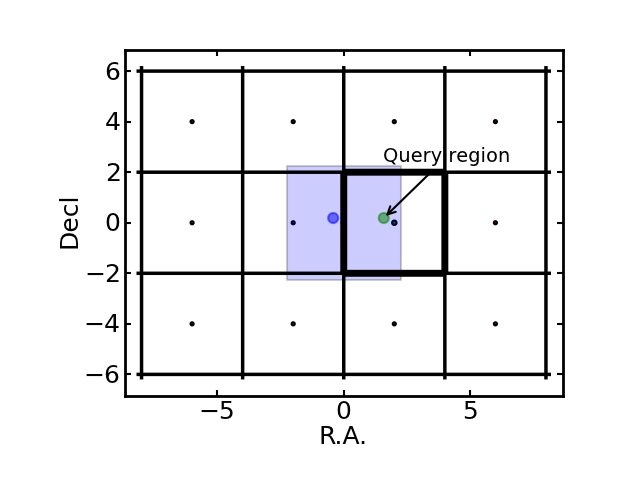
\includegraphics[width=0.5\textwidth]{validation_figures/basicDemo.png}
\caption{The galaxy catalog is replicated (virtually) across the LSST
  footprint using a series of tiles. These tiles correspond to the
  footprint of the galaxy table in the database. Queries are
  transformed using the tile bounding box such that they map to the
  galaxy table. When positions are returned through this query they
  are mapped back to the appropriate sky coordinates using the tile
  bounding boxes.}
\label{fig:galcoverage}
\end{figure}

Solar System sources are the most complicated table in the
database. The typical way to characterize a Solar System object is to
store its 6 orbital elements and propagate the orbit of the source to
the time of the observation. Propagation of all orbits would require a
numerical integration over 11 million sources (for each query). To
accomplish for all sources within the Solar System table for each
query would be computationally prohibitive (requiring 222,000s to
propagate one year into the future). We, therefore, pre-cache the
positions of asteroids within the database and interpolate their
positions based on the time of the observation.

Ephemerides are calculated for all Solar System sources within the
database for a ten year period. The time between ephemerides is
variable and depends on the asteroid population (i.e.\ it is set by
the velocity of the asteroid and the complexity of its orbital
track). For main belt asteroids the positions are stored every two
days together with the Chebyshev polynomial coefficients required to
interpolate between these positions. Figure~\ref{fig:asteroid} shows that,
using a cubic interpolation, asteroid positions are returned with an
rms accuracy of $<1$ mas (sufficient to meet requirement {\it
  Catalogs: Requirements 5}). These cached positions are indexed using
a HTM to speed the spatial lookup. This results in a query for 20,000
asteroids (i.e.\ larger than a full focal plane) requiring 30 ms to
complete.

\begin{figure}[h]
\centering
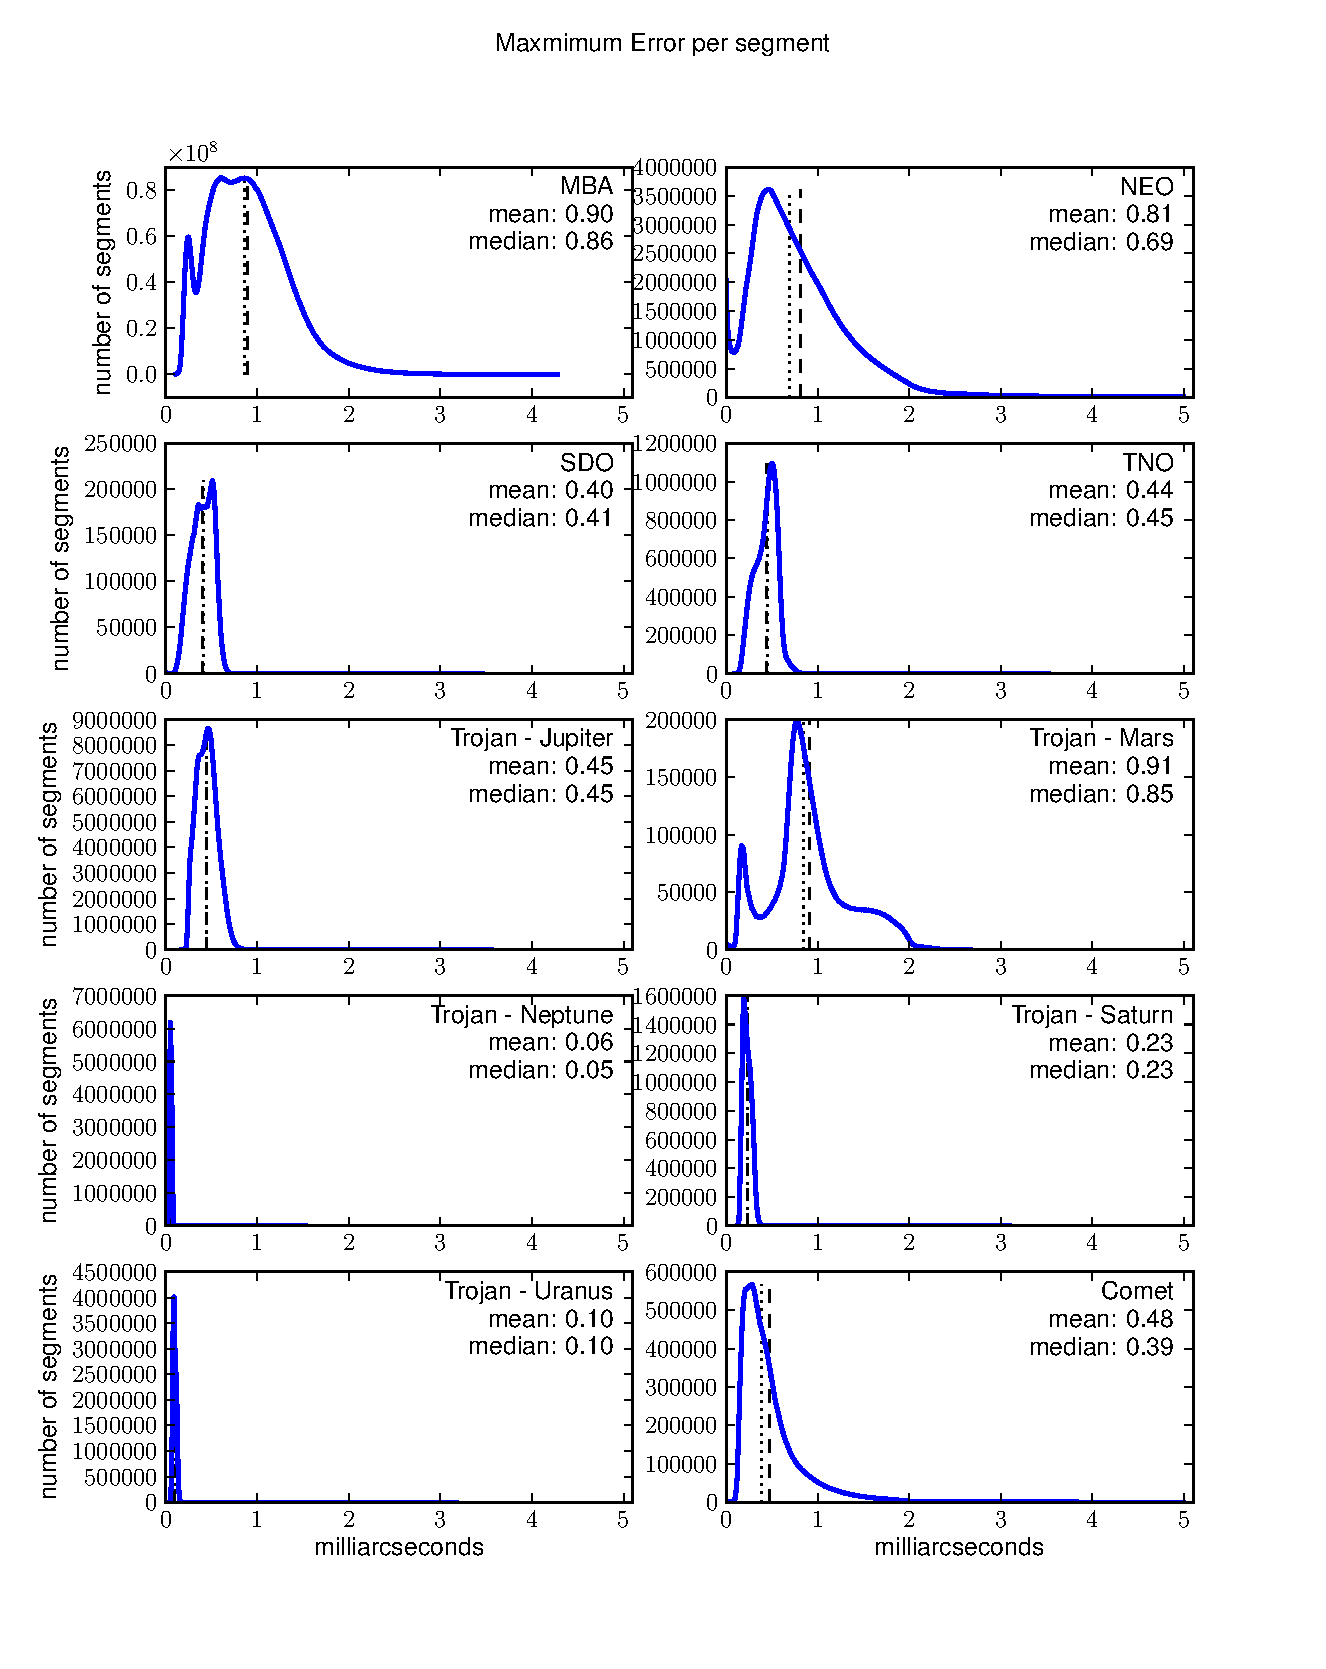
\includegraphics[width=0.65\textwidth]{validation_figures/ErrorHistogramsLinear.pdf}
\caption{The distribution of maximum errors introduced to the orbital
  positions of asteroids due to the adopted interpolation
  scheme. These distributions are given as a function of asteroid
  populations. All populations meet the requirement that the
  interpolation be accurate to an rms of 1 mas.}
\label{fig:asteroid}
\end{figure}


%, it is very slow with so many objects (11
%million total).  In order to keep query times reasonable the objects
%should be indexed so that it is fast to find objects that could
%possibly be within a particular aperture at a given time.  Ideally the
%index would identify exactly (to the precision required by LSST) the
%location of objects that land in the aperture are located at a given
%time.

For all of these sources, the generation of magnitudes and colors, and
the application of time dependent astrometric corrections (e.g.
precession, parallax, proper motion) are calculated using Python
subclasses of the InstanceCatalog object.

\subsubsection{Variable Sources}
The framework is able to support several types of variability:
periodic, stochastic, and repeating.  The variability models used in
the database include:.
\begin{itemize}
\item M-dwarf flares -- full sky
\item AGN/QSOs -- full sky
\item RRly -- full sky
\item Cepheids -- exemplar individuals
\item Eclipsing binaries -- exemplar individuals
\item Am CVn -- exemplar individuals
\item Micro lensing -- exemplar individuals
\end{itemize}
Each type of variability is described by either a parametric model or
an interpolated lookup table (see \S\ref{sec:determine} for a
description of these models).  To date only mono-chromatic variability
has been implemented.
% (see Figure \ref{fig:lcs} for example lightcurves).
%Variable sources are implemented through the InstanceCatalog API
%\citep{XXX}. This API takes the name of the variability model and the
%parameters associated with that model (both of which are stored in the
%database) and modifies the brightness of a source based on the time of
%observation.

\subsection{Catalogs: Requirement 2}

{\it Source characteristics: At high Galactic latitudes the average
  number densities of sources shall be within 20\% and 10\% of the
  observed counts for stars and galaxies respectively (to the
  $5\sigma$ point source coadded depth of the LSST) } \\

%Stellar number densities at Galactic latitudes closer than to the
%plane than $|b| < 30^o$ are difficult to model due to the rising
%density and resulting confusion and deblending issues.  For these
%reasons, the criterion for stellar number counts at low latitudes are
%relaxed to $\pm 30\%$.  For stars where $|b| > 30^o$, the Galfast
%model has been vetted against the SDSS data.  For stars with $|b| <
%30^o$, we quantify the uncertainty in the model by comparing two
%reference models for Galactic structure.  We compare the realization
%of the Galfast model to a realization of the \citet{besancon} model.

\subsubsection{Stars}
We consider five representative fields at varying Galactic latitudes
and at a Galactic longitude of $l=90$.  We compare the number counts
of main sequence stars as a function of $i$-band limiting magnitude
for the Galfast model \citep{juric} (using the composite dust model of
\citet{amores05} normalized to \citet{schlegel98}) to the
\citet{besancon} model (using their standard dust model).  Figure
\ref{fig:scounts_90} shows the cumulative number counts as a function
of magnitude for the Besan\c{c}on (dashed) and Galfast (solid) models
for five values of Galactic latitude.  We also show SDSS counts for two
latitudes ($b=30^{\circ}$, squares, and $b=70^{\circ}$ circles).  For
high glactic latitudes ($|b| >30$), the agreement with the SDSS counts
is best with the Galfast models (with a 13\% difference between
Galfast and SDSS at the limit of the SDSS data). For low Galactic
latitudes there is insufficient observational data to constrain the
Galfast of Besan\c{c}on models.

In Figure \ref{fig:sratio_90} we show the ratio of Besan\c{c}on counts
to Galfast counts for the five test fields.  The dashed lines are the
$\pm30\%$ limits for the low latitude sizing model constraints and the
dash-dot lines are the $\pm20\%$ limits for the high latitude limits
requirements.  For all Galactic latitudes $b<-30$ the Besan\c{c}on and
Galfast models disagree at $>$20\% requirement for stellar
densities. For low Galactic latitudes ($b=-10$) the Besan\c{c}on and
Galfast models are in good agreement (i.e.\ within the 20\%
requirement on stellar number densities) .

%In the case directed toward the galactic bulge, all fields meet the
%requirements at the co-added depth except for $b=-10$.  At the nominal
%single epoch depth, the $b=-10$ case fails and the $b=-30$ case misses
%the $\pm20\%$ requirement, but makes the $\pm30\%$ requirement.
% PUT THIS BACK IN?

%For the high latitude fields away from the Galactic bulge, the
%deviation from the Besan\c{c}on model is within the stated
%requirement.  The $b=-10$ case, the number counts from Galfast
%significantly under predict relative to the Besan\c{c}on model.  The%
%$b=-30$ case shows similar, though not as drastic, under prediction
%and misses the requirement for all but the faintest magnitudes and
%even then only meats the $\pm30\%$ requirement.

%We repeated this analysis using the GALFAST dust model and the results do not change significantly


\begin{figure}[h]
\centering
\begin{subfigure}[b]{0.45\textwidth}
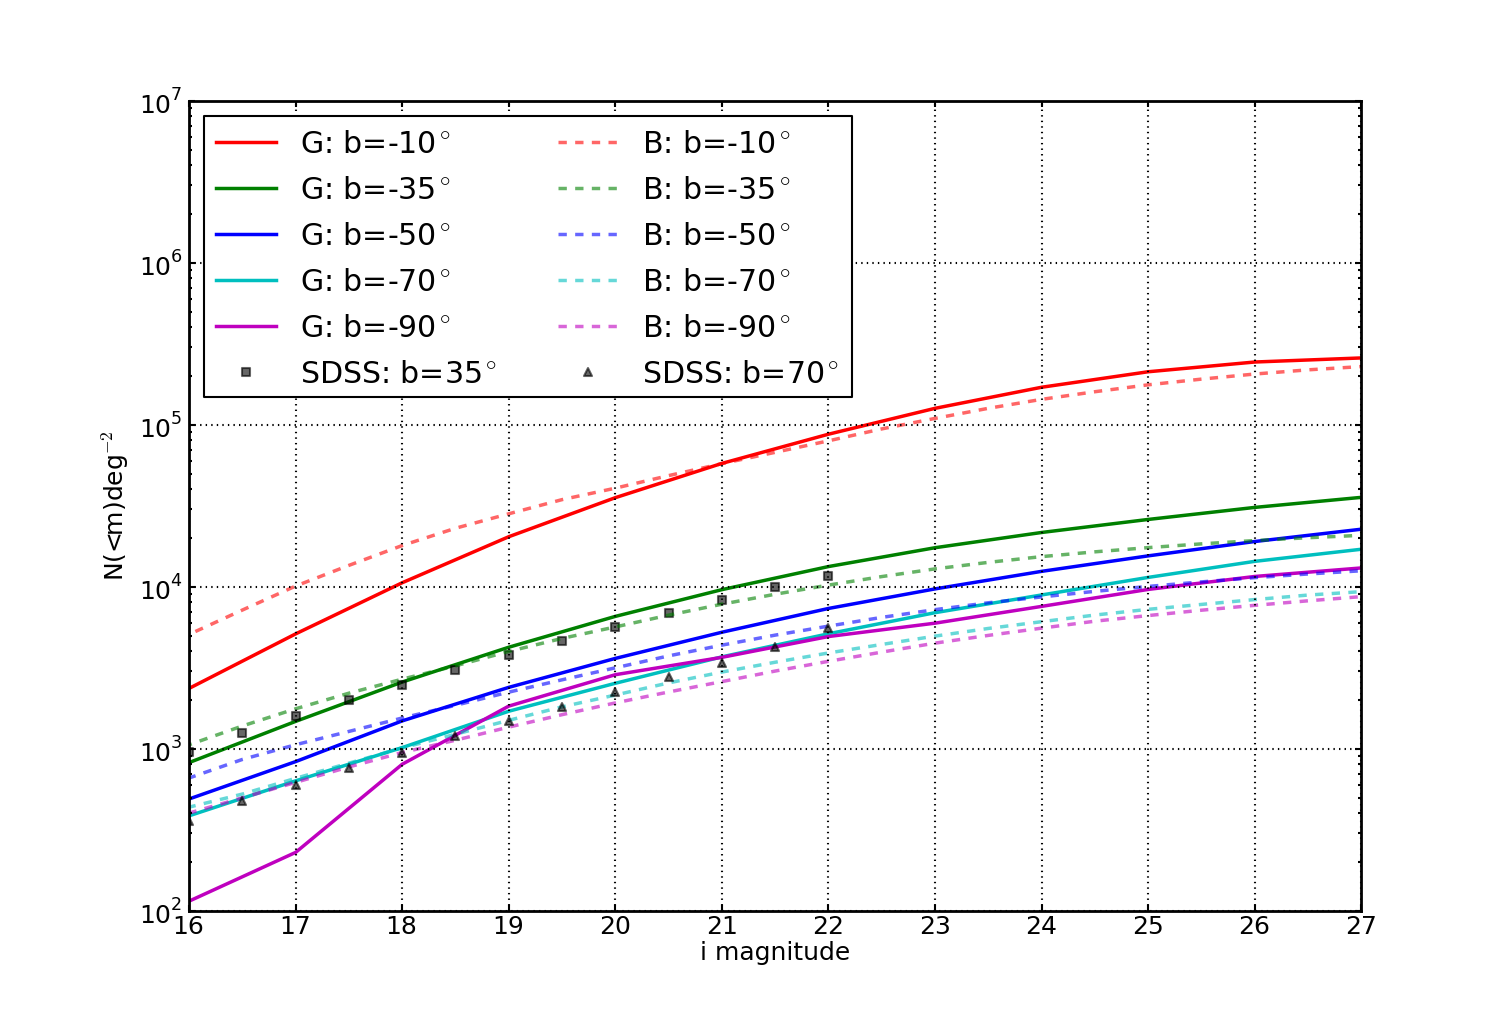
\includegraphics[width=\textwidth]{validation_figures/cumulative_stars_90_besancon_dust.png}
\end{subfigure}
\begin{subfigure}[b]{0.45\textwidth}
\centering
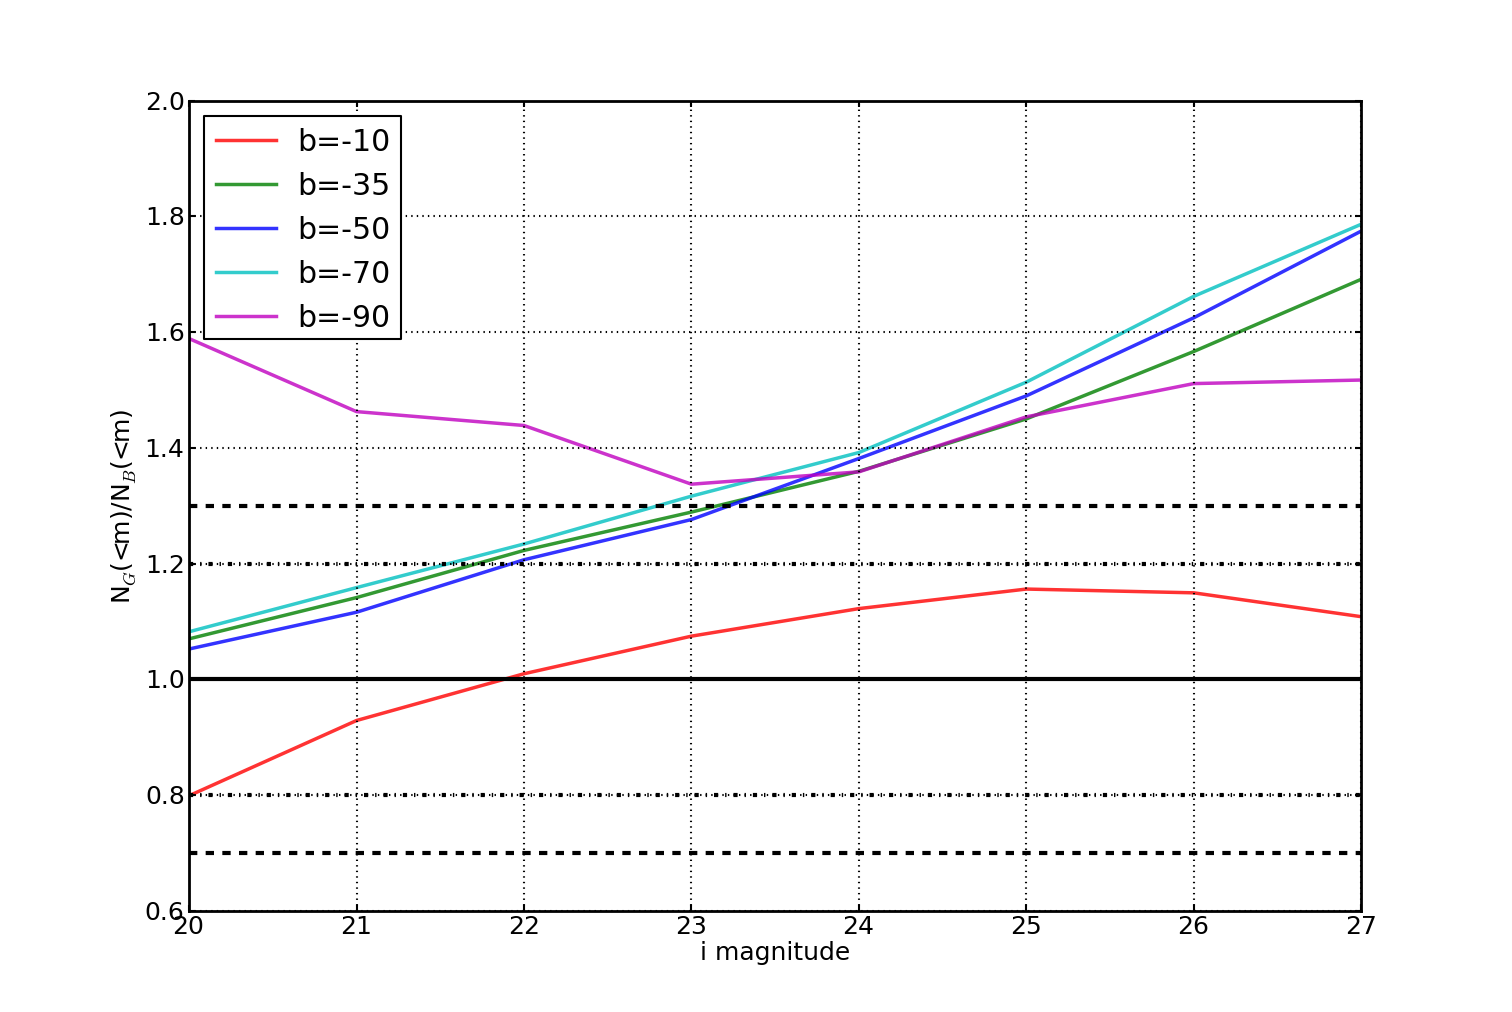
\includegraphics[width=\textwidth]{validation_figures/cumulative_ratio_stars_90_besancon_dust.png}
\end{subfigure}
\caption{Cumulative counts of stars from the Besan\c{c}on (dashed) and
  Galfast (solid) models for 5 representative fields toward
  l=90$^o$. The left panel shows the counts from these models and the
  SDSS and the right panel the ratio of the Besan\c{c}on and Galfast
  models. For $b<-30^{\circ}$ and $i<22$, the SDSS counts are 13\%
  lower than the numbers predicted by the Galfast model.}
\label{fig:scounts_90}
\label{fig:sratio_90}
  \end{figure}

\subsubsection{Galaxies \label{sec:galaxycounts}}

The left panel of Figure \ref{fig:gcounts} shows a comparison of the
cumulative galaxy counts in CatSim to a compilation of observations
provided by Metcalfe et al. (see {\tt
  http://ls.st/fus}).  This
comparison is undertaken in the $i$ band to minimize the effects of
dust extinction which are somewhat uncertain in the Metcalfe
compilations.  A single transform of I$_{kc}$ = i$_{AB}$ - 0.6 has
been applied to the Metcalfe magnitudes to take them from the
Kron-Cousins photometric system to the SDSS AB photometric system \citep{ellis07}.

The right panel of Figure \ref{fig:gratio} shows the ratio of the
cumulative counts taken from the simulations to a polynomial fit to
the cumulative counts derived from the Metcalfe data.  The error bars
are estimated from the published uncertainties on the Metcalfe galaxy
number counts. The requirement on galaxy number densities is that they
agree within $\pm10\%$ of the observed counts (to a coadded i-band
depth of 26.8). This requirement is set due to the variance in the
counts of galaxies at faint magnitudes (due to the small areal
coverage of galaxy surveys at these depths).  For magnitudes
$20.25<i<25.75$ the simulated galaxy catalog meets the LSST
requirements.  For brighter magnitudes the simulated catalogs
over-predict the galaxy counts by up to 25\%. This discrepancy is to be
expected as the volume sampled by the simulated galaxies (covering
$4.5^o \times 4.5^o$) is small relative to the observations and the
cosmic variance in the simulated data will be large. For magnitudes
fainter than $i>25.75$ the galaxy counts fail to meet the number
density requirement; deviating by up to 13\% from the observed counts.

% We have
%taken their compilations from: {\tt
%  http://star-www.dur.ac.uk/~nm/pubhtml/counts/idata.txt} accessed on
%06/01/2013. 

\begin{figure}[h]
\centering
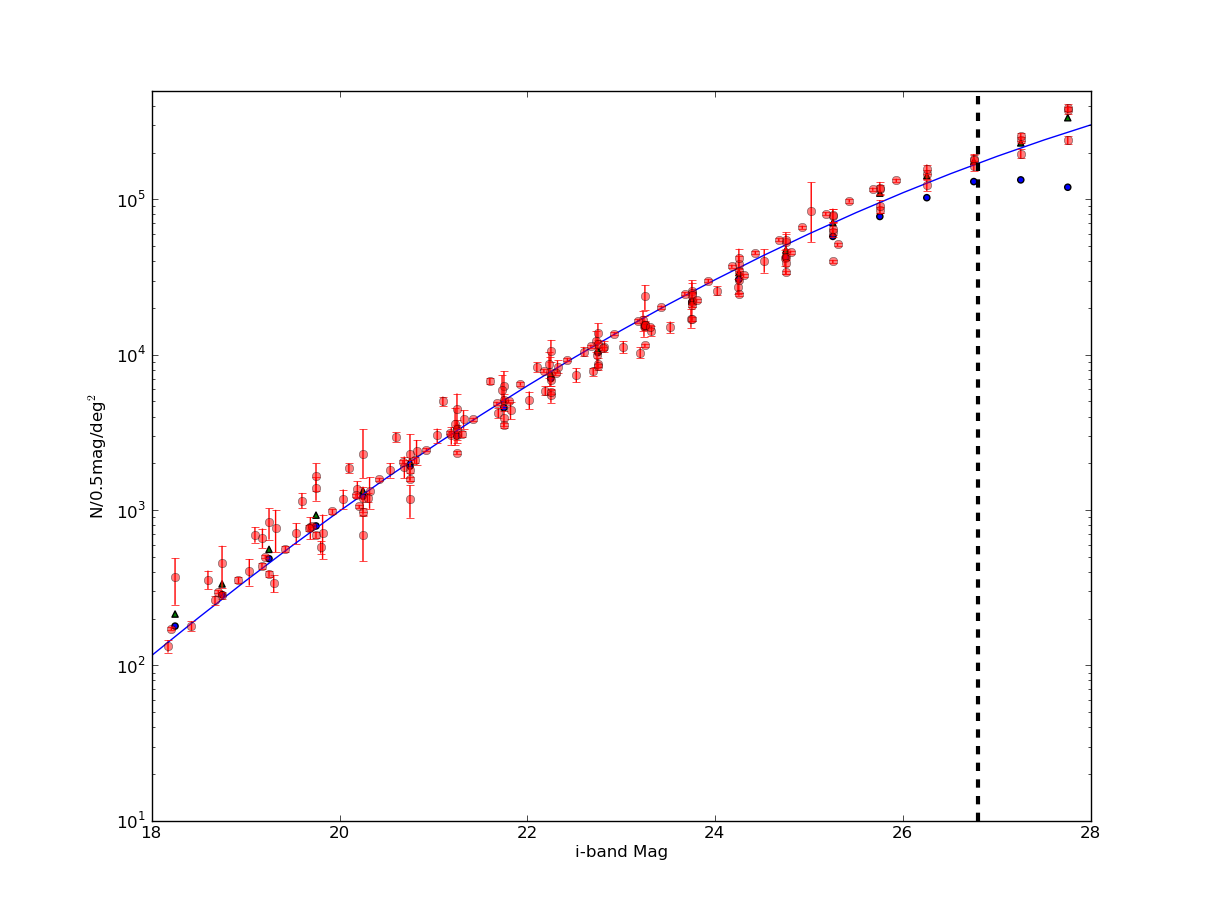
\includegraphics[width=0.45\textwidth]{validation_figures/Ngals-i.png}
\hfil 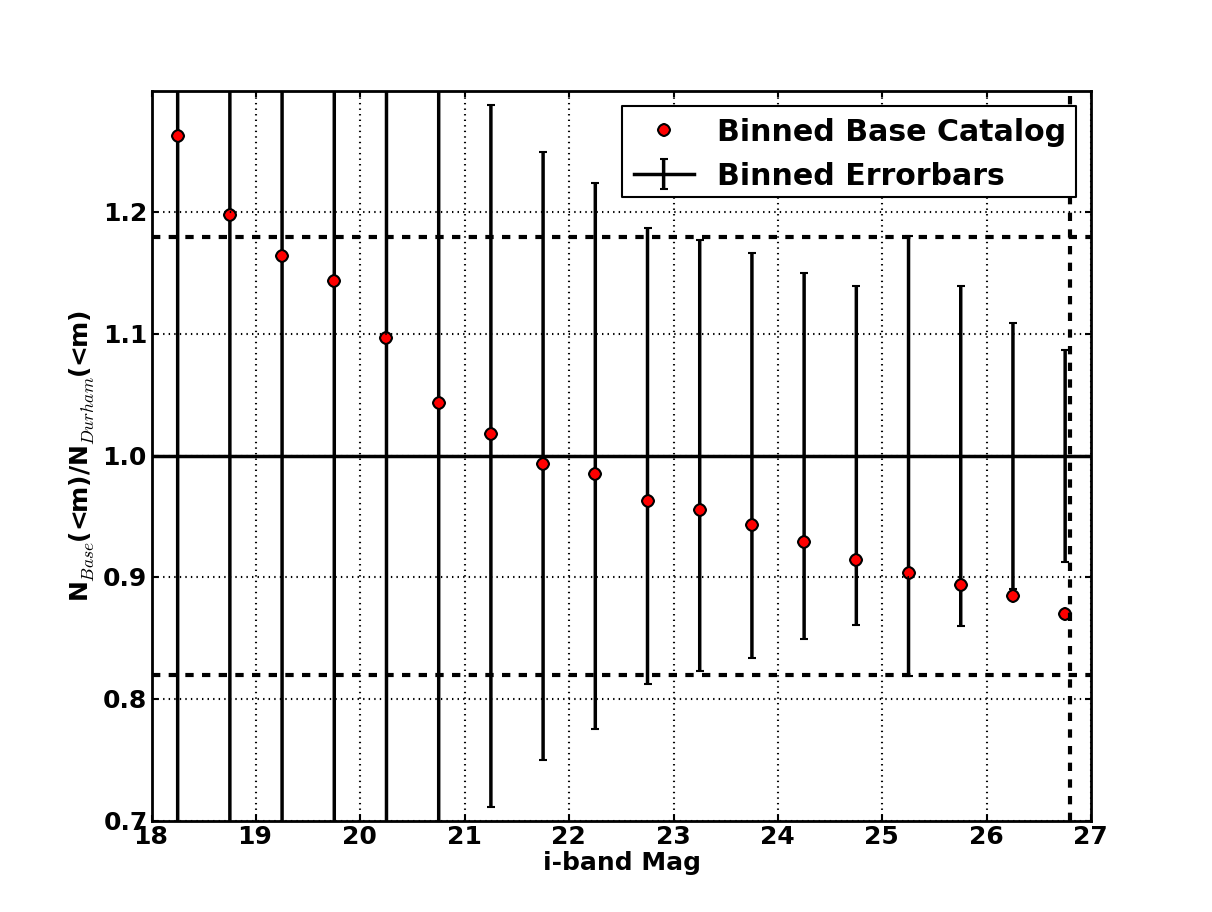
\includegraphics[width=0.45\textwidth]{validation_figures/CumulativeFraction_i.png}
\caption{A comparison of the Metcalfe galaxy number counts (symbols)
  to those derived from the simulated catalog \label{fig:gcounts}. The
  left panel shows the differential counts and the right panel the
  ratio of the cumulative counts. Error bars are from derived from
  those published by the individual surveys. \label{fig:gratio}
The vertical dashed line represents the
  5$\sigma$ magnitude limit for galaxies.}
\end{figure}

\subsubsection{Ramifications of missing the number density requirements}

For stellar counts away from the bulge, the Galfast model matches the
observed densities of stars to the limit of the SDSS data. Comparison
with the Besan\c{c}on model, however, shows a discrepancy of over 30\%
between the predicted counts for latitudes $b<-35$ (and $i>23$).  In
all such cases the LSST model from Galfast over-predicts the densities
of stars compared to Besan\c{c}on. While it is clear that there is
significant uncertainty between the models, the fact that Galfast
predicts a higher density of stars than Besan\c{c}on and that it
reproduces the densities of stars in the SDSS, minimizes the risk that
the compute and sizing model will be under resourced (i.e.\ it risks
over provisioning of the compute resources).

For lower Galactic latitudes ($b=10$ ) and away from the bulge, there
is good agreement between the stellar structure models (see
Figure~\ref{fig:gratio}) but limited observational data to validate
either model. Toward the bulge the stellar densities disagree by nearly
a factor of three at $b=-10$ with Besan\c{c}on predicting a lower density of
stars. This is outside of both the simulation requirements and the
margin for the sizing model but is only for a small part of the survey
volume (see DMR-21 in the DM Risk Register for the proposed actions in
response to this risk).  

The validity of the Besan\c{c}on as ground truth in the plane of the
galaxy is not obvious.  In fact, SDSS and Galfast star counts agree
surprisingly well at low galactic latitudes (M. Juri\'{c}, private
communication).  Part of the current disagreement may arise due to the
fact that the Besan\c{c}on models are drawn from distributions with
binary corrections applied while the Galfast model does not produce
unresolved binary systems as multiple objects in the catalogs (i.e.\
the Galfast models should under-predict relative to the Besan\c{c}on
by approximately the unresolved binary fraction).  To resolve these
questions, for bright magnitudes, a comparison will be taken with
existing survey data including those from Pan-STARRS.

For galaxy counts, the number counts fail to meet requirements for
magnitudes $i>25.75$. At the limiting depth of the coadded survey
these counts are less than 2$\sigma$ from the observed counts (where
$\sigma$ is the observational uncertainty due to a combination of shot
and cosmic variance). While the galaxy simulations are within the
bounds set by Data Management for the sizing model (i.e.\ $<30$\%)
this issue will be resolved by re-cloning the galaxy data to match
deeper number count models.

\subsection{Catalogs:  Requirement 3}

{\it Size, ellipticity, and redshift distributions of galaxies shall
  be representative of those observed by extant space and ground-based
  telescopes and, for a fiducial image quality of 0.72 arcsec,
  deviations from the observed distributions shall contribute $<20$\%
  of the observed effective density of galaxies, n$_{eff}$, used in
  weak lensing samples (assuming a fiducial value of n$_{eff} =
  28$ galaxies per arcmin$^2$)}\\


The ability to use gravitational weak lensing to constrain
cosmological parameters is dependent on $n_{eff}$; the effective
density of galaxies on the sky that are resolved sufficiently such that
shear can be measured from the shape of a galaxy. The size of
$n_{eff}$ depends on the inherent shape noise of the galaxies, the
size distribution of the galaxies relative to the size of the PSF, and
the signal-to-noise of the observations.  Following the methodology of
\citet{chang} we calculate $n_{eff}$ for the distributions in the base
galaxy catalog.  In summary, we use Equation 9 to calculate $n_{eff}$:
\begin{equation}
n_{eff} = \frac{1}{\Omega}\sum^N_i\frac{\sigma^2_{SN}}{\sigma^2_{SN}+\sigma^2_{m,i}}
\end{equation}
where $\sigma_{SN}$ is the intrinsic shape noise, $\sigma_{m,i}$ is
the shape measurement uncertainty for the i$^{th}$ galaxy, and $N$ is
the number of galaxies in the sample. The shape noise is derived from
the ellipticity distribution of the galaxies with $\sigma_{SN} = 0.26$
\citep{chang}.  The measurement noise can be approximated using
Equation 13 of \citet{chang}:
\begin{equation}
\sigma_m(\nu,R) = \frac{a}{\nu}\left[1+\left(\frac{b}{R}\right)^c\right]
\end{equation}
where $\nu$ is the signal-to-noise ratio of the source, and
$R=\frac{r_{gal}^2}{r_{PSF}^2}$ is the area of the galaxy relative to
the point spread function.  We adopt values from \citet{chang} of
(a,b,c) = (1.58,5.03,0.39), and assume a fiducial PSF size of 0.72
arcsec. We use an estimate for the limiting magnitude for the co-added
images of 26.7.  This value reproduces the values presented in
\citet{chang}.  We expect the measured value of the limiting depth to
be brighter than the SRD value of 27.5 in r because the SRD value is
defined for dark sky at zenith while the \citet{chang} data have a
distribution of airmass and sky brightness.  
%The fact that
%the measurements are on extended sources also contributes to the best
%fit value being brighter than the nominal SRD value.  
For our comparison we define a ``Gold Sample'' of galaxies with $i <
25.3$ (see \citealt{LSSTScienceBook}).  For each galaxy, $r_{gal}$ is
calculated from the flux ratio of the bulge and disk components as
well as the effective half light radii of each component (see Appendix
B in \citet{chang} for a derivation of this calculation).

Using this framework, we test the sensitivity of the measured
$n_{eff}$ against our assumptions for the ellipticity, size,
magnitude, and redshift distributions of the galaxies in the universe
model.  For all calculations that follow we use the $k=1$ criterion of
\citet{chang}; meaning that galaxies with $\sigma_m < \sigma_{SN}$ are
culled from the sample. This assumes that no improvement has been made
in the measurement of shear over current techniques.  

The galaxy shape noise distribution has been measured by the COSMOS
project \citep{cosmos} and, to first order, the dependence of
$n_{eff}$ on the shape of the distribution can be expressed in terms
of the variance of the ellipticity distribution. The dependence of
$n_{eff}$ on apparent magnitude arises due to the steepness of the
galaxy number counts. As is shown in Figure \ref{fig:neffvm}, however,
due to the decrease in signal-to-noise of the sources there is a sharp
cut-off in the value of $n_{eff}$ at $i=25.0$.  Given this, galaxy
redshift distributions must agree with observations to a limiting
magnitude of $i=25.0$ to ensure an accurate mapping between physical
and angular size.  Finally, the size distribution of the combined two
component galaxy model must reproduce the measured distributions.

The ellipticity distribution is measured from the base catalog by
sampling the composite Sersi{\'c} (bulge and disk together) using the
ellipsoid parameters and the appropriate flux ratio for each galaxy.
The moments are measured and ellipticities calculated using the
definitions in \citet{chang}.
\begin{equation}
\epsilon_1 = \frac{I_{11}-I_{22}}{I_{11}+I_{22}+2\sqrt{I_{11}I_{22} - I^{2}_{12}}},~
\epsilon_2 = \frac{2I_{12}}{I_{11}+I_{22}+2\sqrt{I_{11}I_{22} - I^{2}_{12}}}
\end{equation}
where $\epsilon_1$ and $\epsilon_2$ are the $x$ and $y$ components of
the ellipticity and $I_{11}$, $I_{12}$, $I_{22}$ are the variance and
covariance of the moments of the light distribution.

The measured variance in the ellipticity distribution of the galaxies
in the simulation catalog is $\sigma_{SN} = 0.26$; identical to that
reported by \citet{chang}. The shape differs slightly from the COSMOS
distribution with a broader tail and wider central component. (see
Figure \ref{fig:e_hist}).  As shown in the bottom two panels of
Figure~\ref{fig:e_hist} these slight variations in ellipticity
distribution do not impact the measured value of $n_{eff}$.  The
bottom left panel of Figure~\ref{fig:e_hist} shows a distribution that
is too wide to meet the $n_{eff}$ requirement, and the bottom right
panel of Figure~\ref{fig:e_hist} shows a distribution that is too
narrow to meet the requirement.

\begin{figure}[h]
\centering
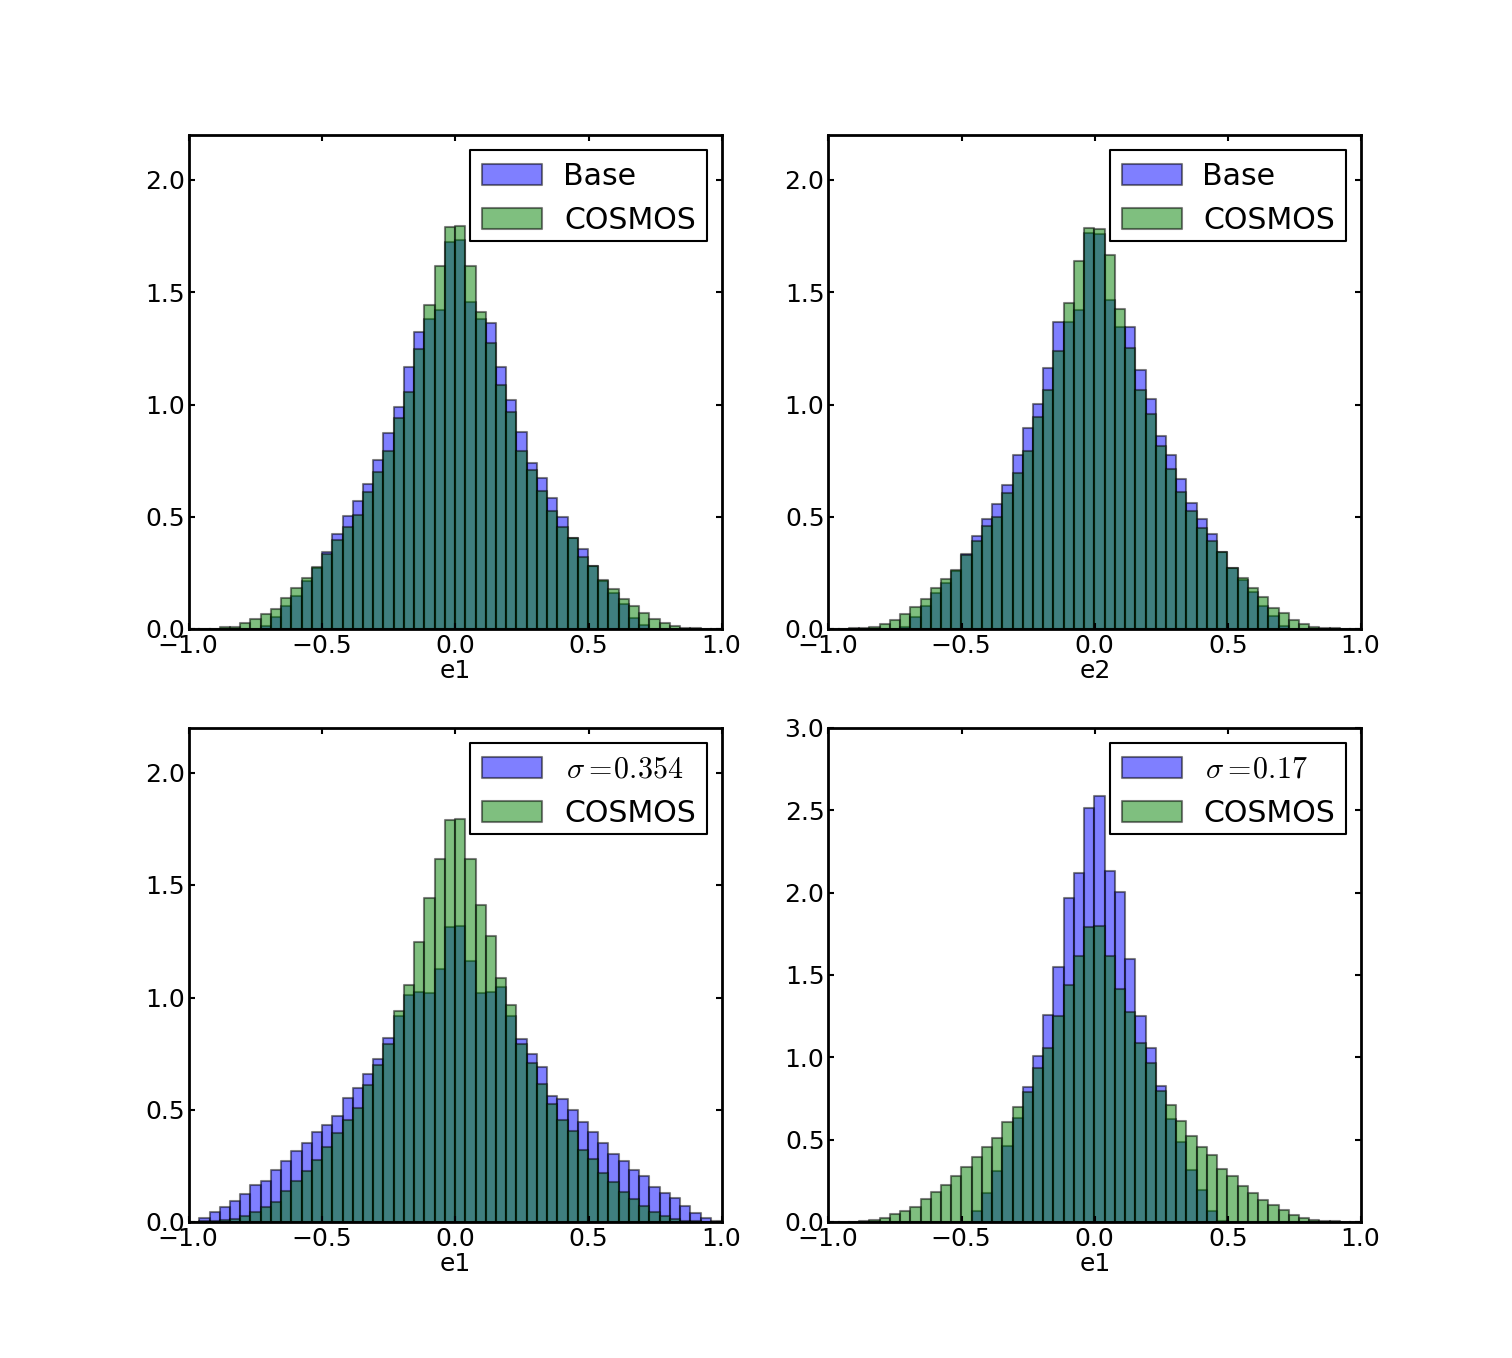
\includegraphics[width=0.5\textwidth]{validation_figures/e_hist.png}
\caption{The top two panels are the histograms of e1 and e2 values for
  the base catalog and COSMOS sample.  These distributions are for
  objects with $20.0 < i < 25.0$. The lower two panels show
  ellipticity distributions that are too broad (left panel) or too
  narrow (right panel) relative to the $n_{eff}$ requirements.}
\label{fig:e_hist}
\end{figure}

For completeness, in Figure \ref{fig:nofz18_24}, we show the agreement
between simulated and observed \citep{coil04} redshift distributions
for one magnitude bin intervals from $i=18$ to $i=24$.  As shown in
\ref{fig:neffvm} galaxies with $i > 25$ do not contribute significantly to $n_{eff}$.

\begin{figure}[h]
\centering
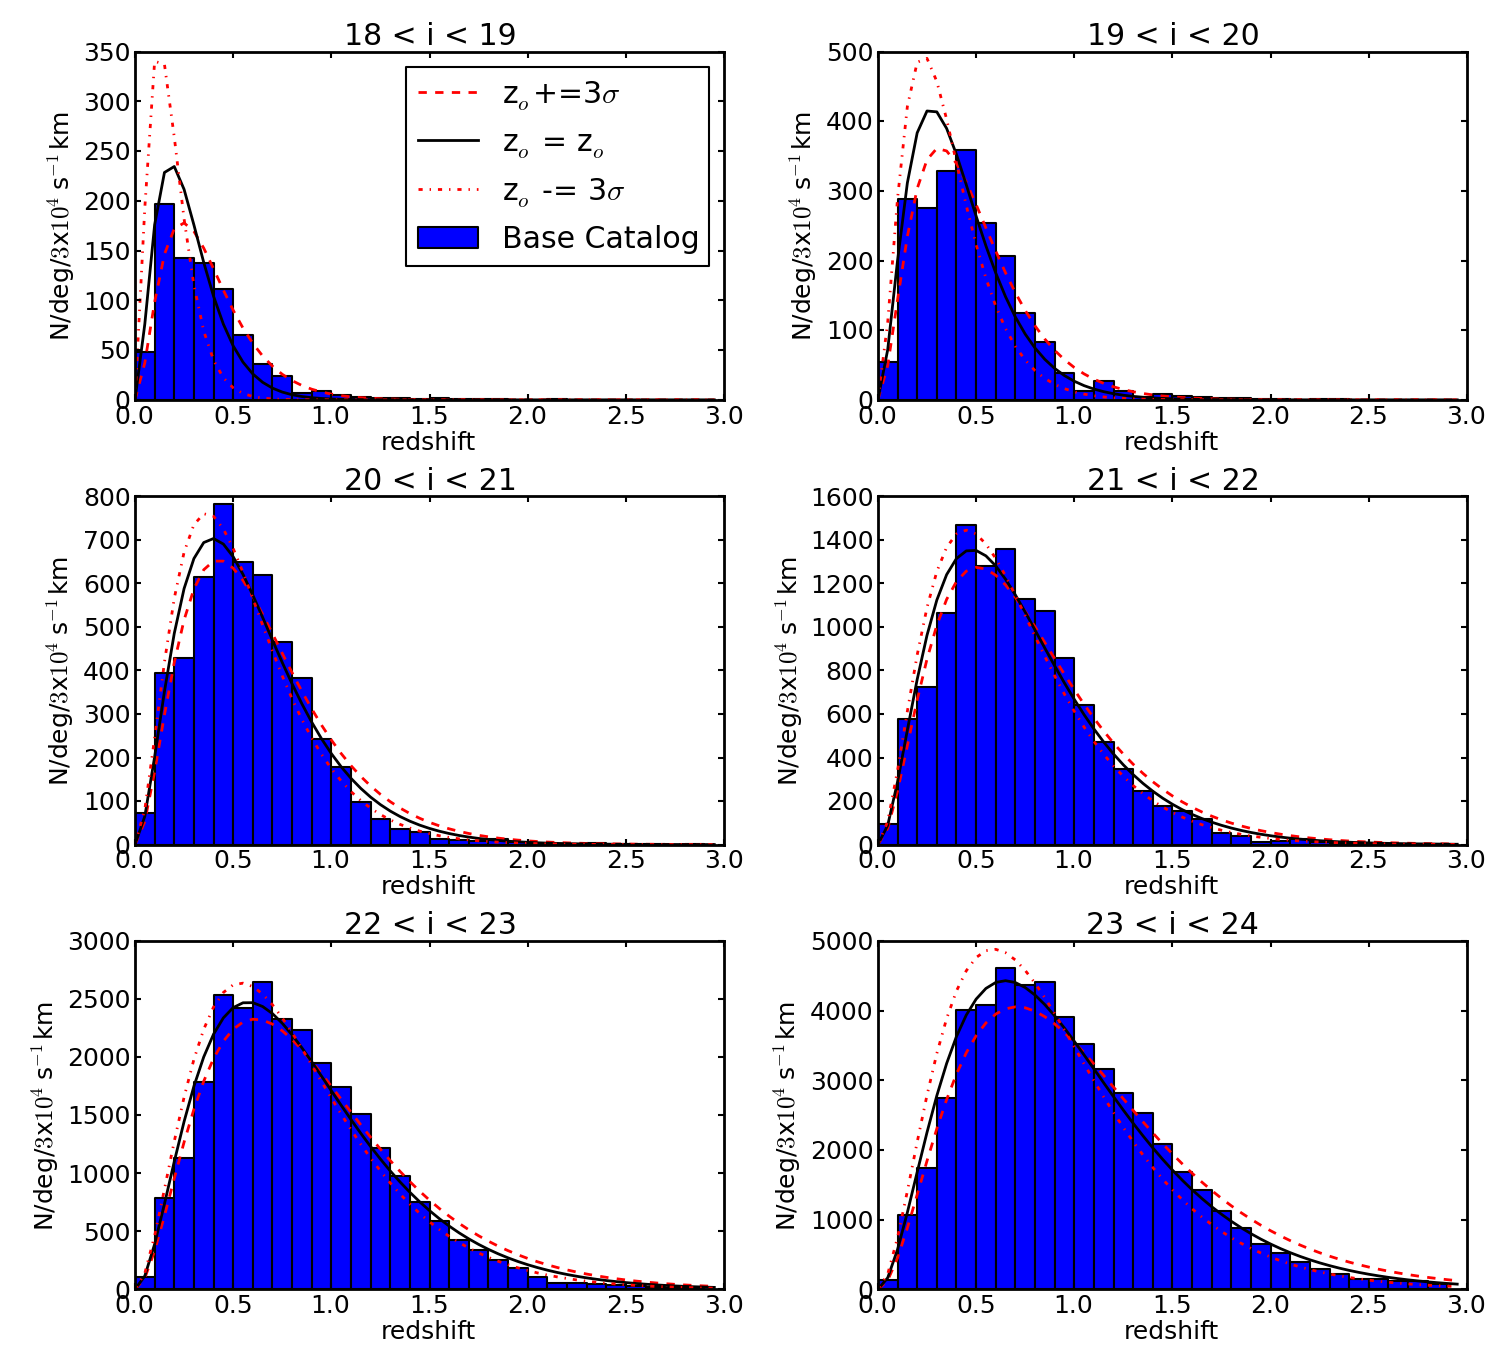
\includegraphics[width=0.5\textwidth]{validation_figures/Nofz_18_24.png}
\caption{The blue histogram in each panel is the measured N(z) for one
  magnitude bins from $18<i<24$.  Over-plotted is the empirical
  distribution from \citet{coil04} normalized to the area of the
  measured distribution.  The dashed and dotted red lines show what
  happens if the governing parameter for the \citet{coil04}
  distribution, $z_o$, is over or under predicted by $3\sigma$
  respectively.\label{fig:nofz18_24}}
\end{figure}
%\begin{figure}
%\centering
%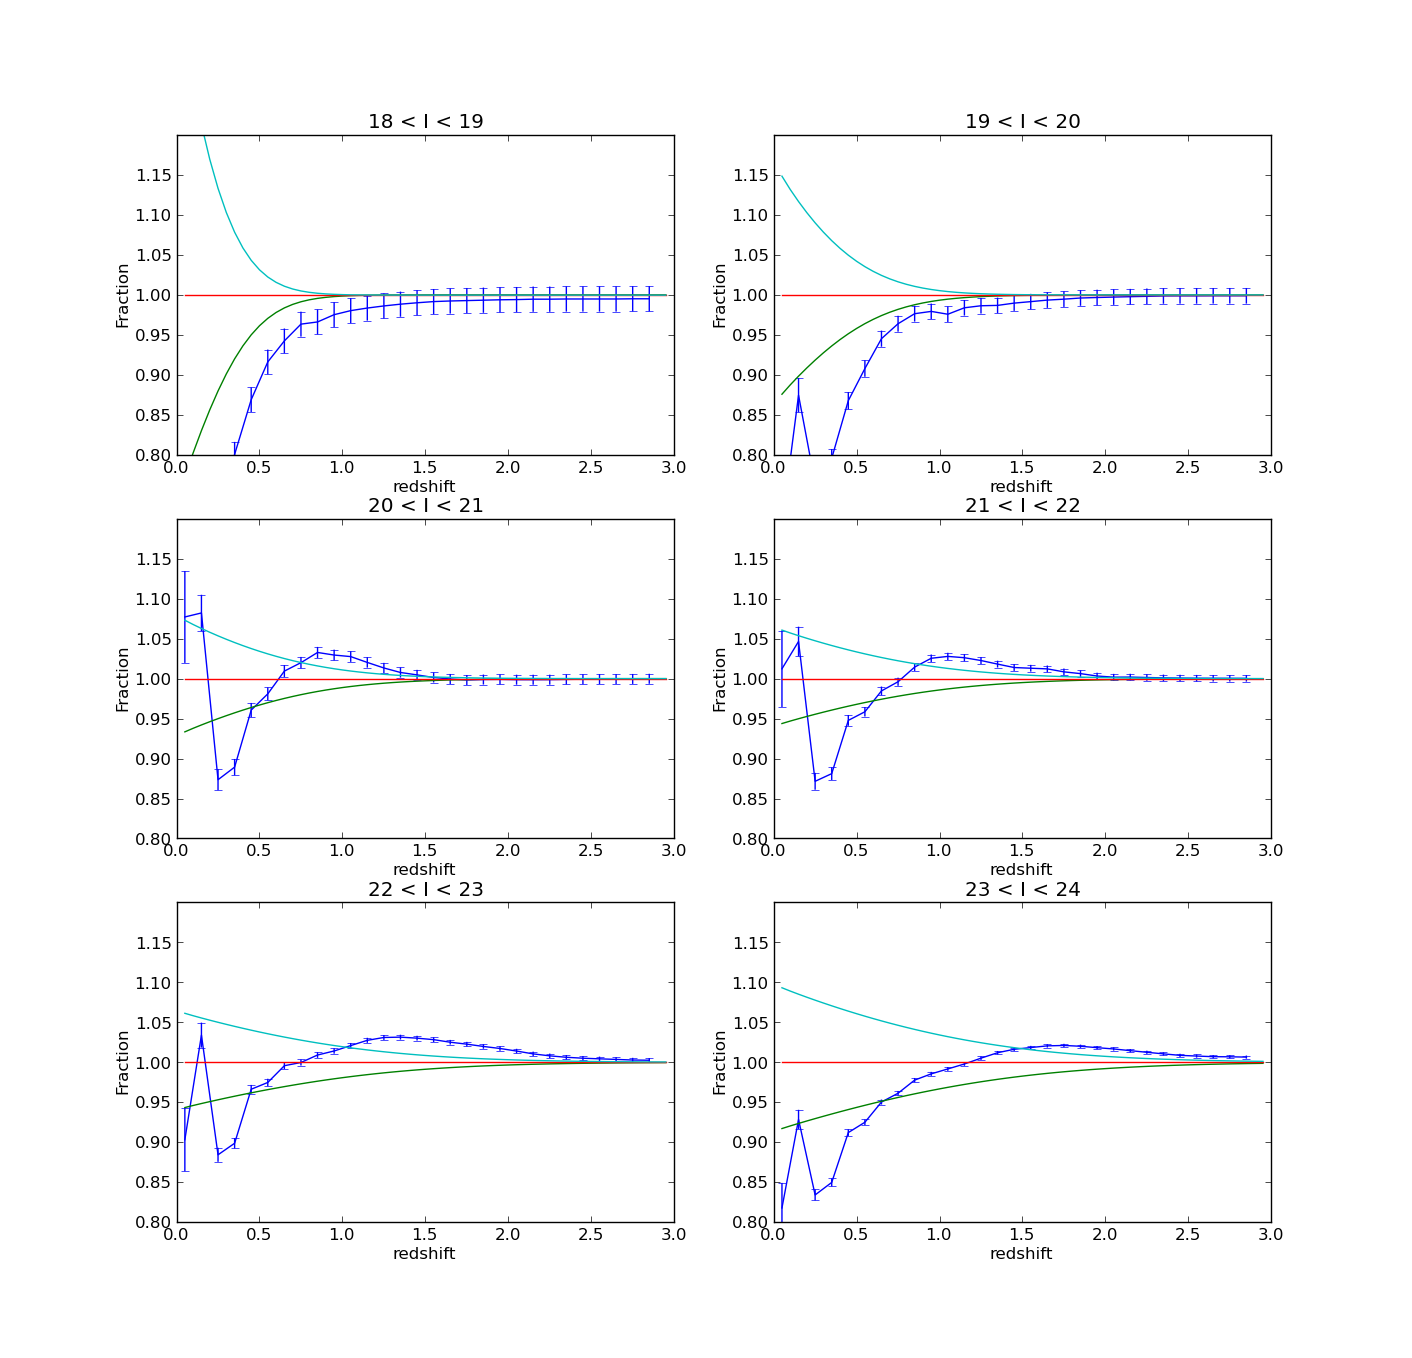
\includegraphics[width=5in]{validation_figures/Nofz_CumulativeFraction_18_24.png}
%\caption{N(z) for 18 to 24 with distribution from \cite{coil}\label{fig:nofz18_24_ratio}}
%\end{figure}
%\begin{figure}
%\centering
%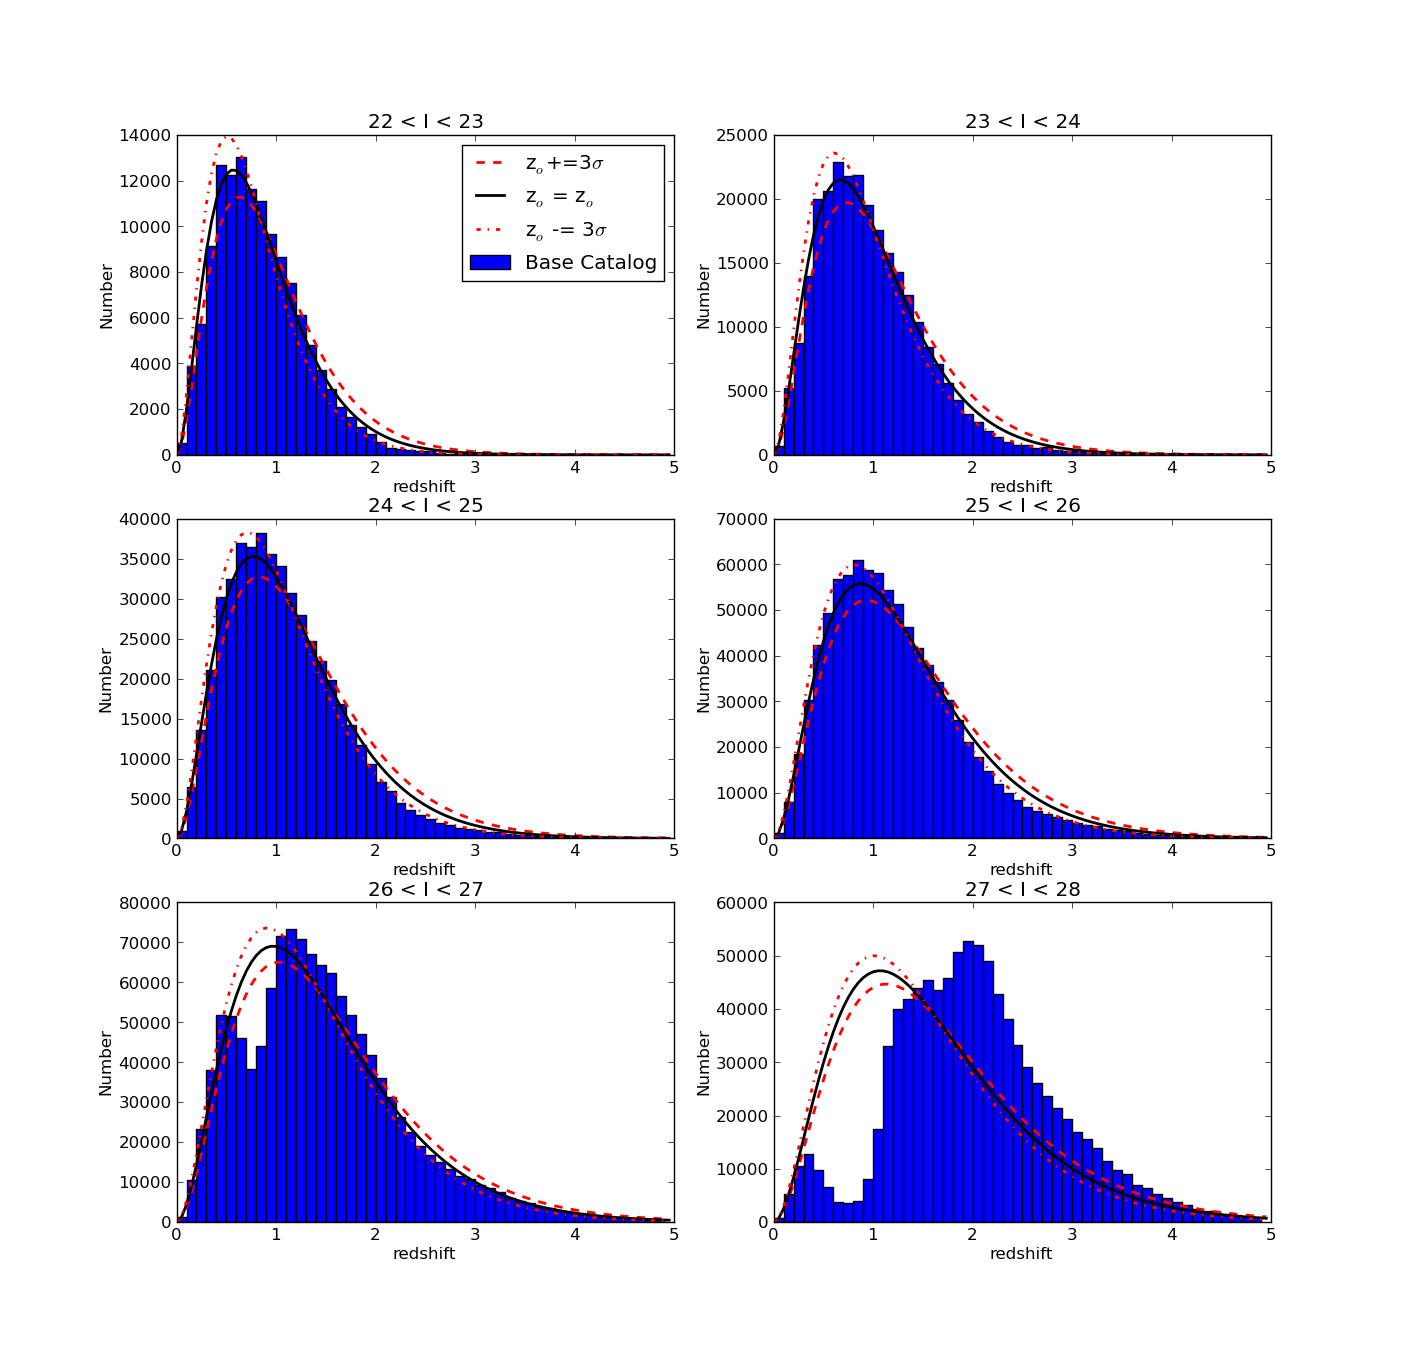
\includegraphics[width=5in]{validation_figures/Nofz_coil_22_28.png}
%\caption{N(z) for 22 to 28 with distribution from \cite{coil}\label{fig:nofz22_28}}
%\end{figure}
%\begin{figure}
%\centering
%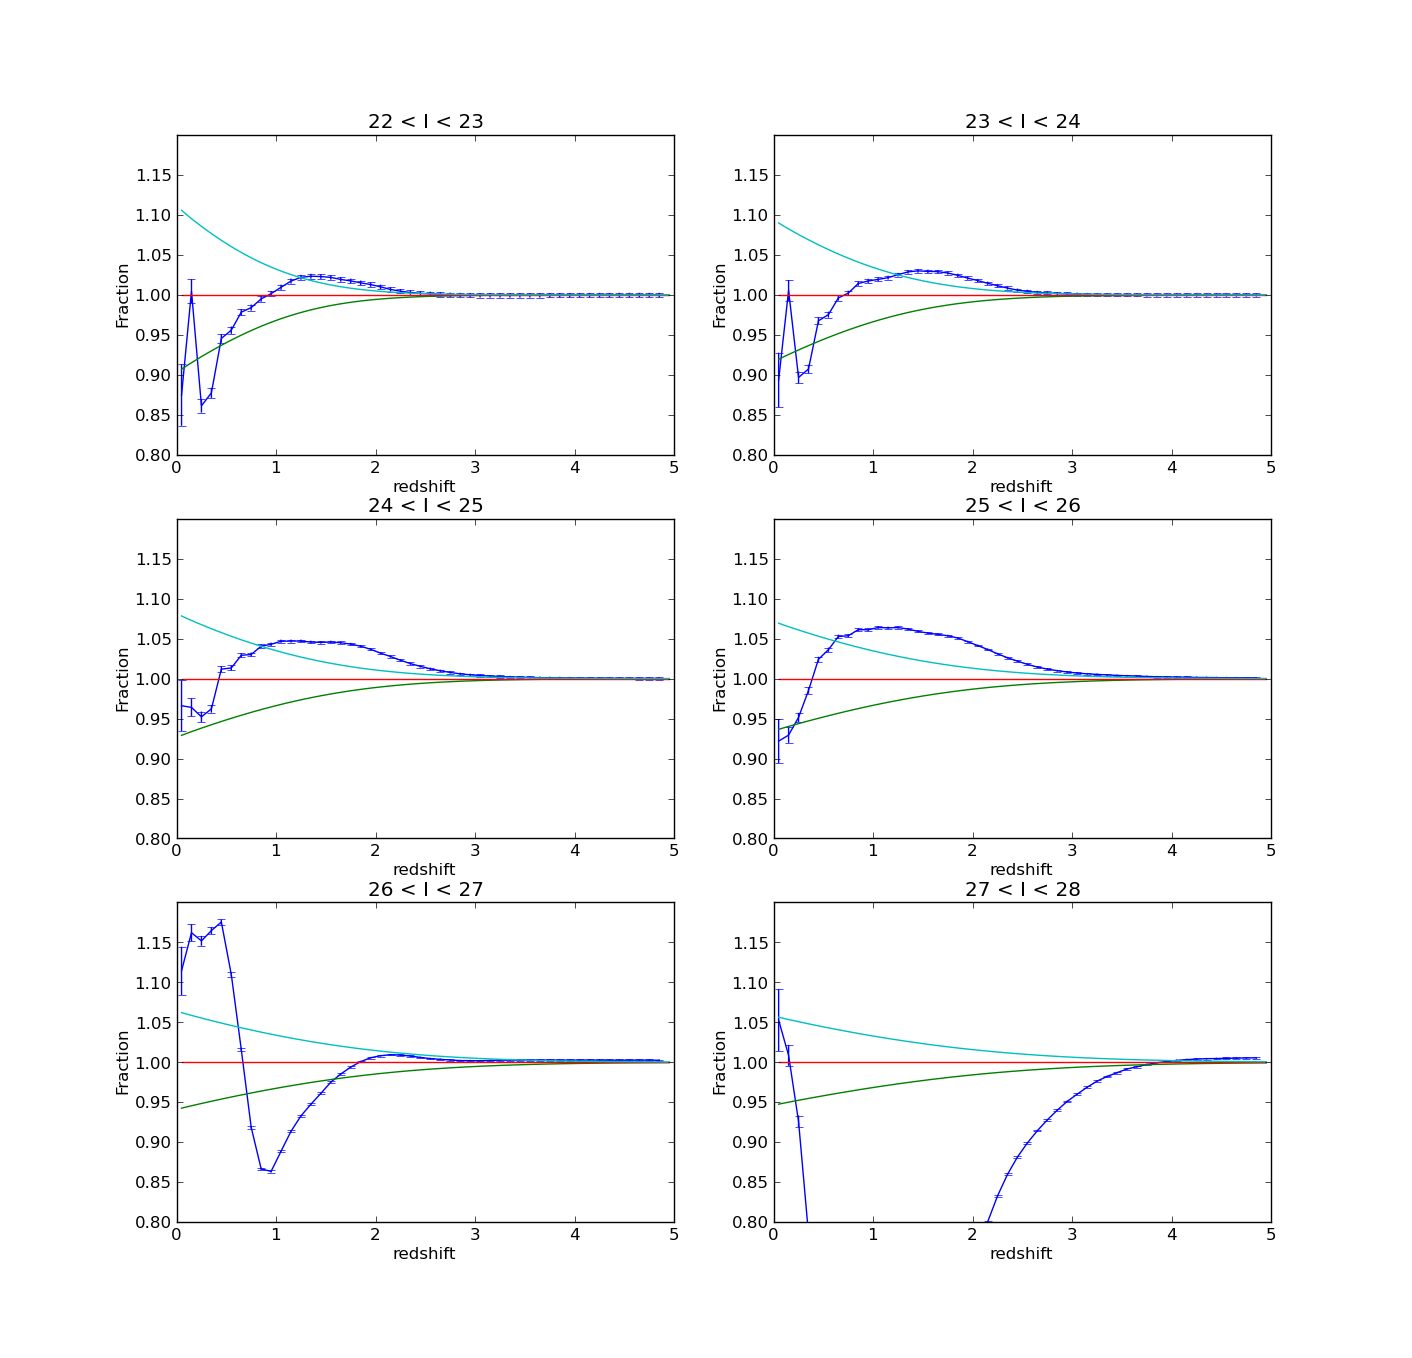
\includegraphics[width=5in]{validation_figures/Nofz_CumulativeFraction_22_28.png}
%\caption{N(z) for 22 to 28 with distribution from \cite{coil}\label{fig:nofz22_28_ratio}}
%\end{figure}
\begin{figure}[h]
\centering
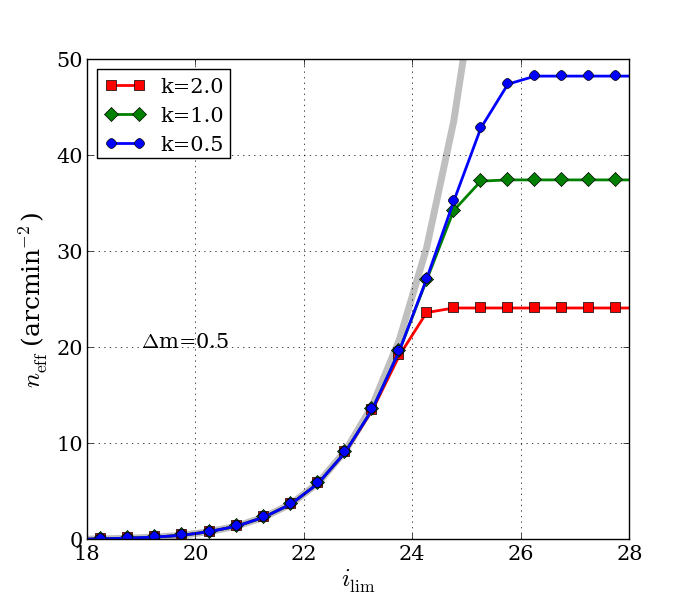
\includegraphics[width=0.5\textwidth]{validation_figures/neff_m_ir.png}
\caption{$n_{eff}$ as a function of i-band limiting magnitude.  Even though the the density of galaxies is going up steeply, the 
size of the galaxies relative to the PSF is falling off quickly enough that galaxies fainter the $i=25$ don't contribute much to $n_{eff}$.\label{fig:neffvm}}
\end{figure}


\subsubsection{Galaxy radii measurements}
There are many definitions of galaxy size: half light radius, first
moment radius, second moment radius, Petrosian radius, Kron radius,
etc.  For the validation of the galaxy size distributions we utilize
data from the COSMOS Advanced Camera for Surveys catalog
\citep{cosmos} as it extends to depths greater than $i=24.5$, is of
higher resolution than ground-based data (i.e.\ with an image quality
of $<0.1$ arcsec), and covers a representative area of the sky (2
deg$^2$). The COSMOS catalog reports both the second moments and the
half light radius.

One concern in comparing observed and model radii is that the base
catalog is effectively infinite signal-to-noise, whereas the
measurements from COSMOS are not.  We, therefore, consider the impact
of the S/N on the derived sizes in order to define the appropriate
measure to use for comparison. We model the effects of signal-to-noise
on the half-light and second moment radii by truncating the Sersi{\'c}
profiles at a specified radius (i.e.\ reproducing the effect of the
light profile dropping below the noise in the image).  We truncate the
profiles at the following multiples of the half light radius,
$R_{hl}$: $1.33R_{hl}, 1.78R_{hl}, 3.16R_{hl}, 10R_{hl},
$ and $100R_{hl}$.

Figure~\ref{fig:size_hist} shows the effect of progressively
decreasing the signal-to-noise of a light profile.  As the
signal-to-noise decreases the peak and width of the distributions of
half light and second moment radii decrease (see Figure
\ref{fig:mom_hl_line}).  Going from $100R_{hl}$ to $10R_{hl}$, the
mean of the second moment radius distribution decreases by $14\%$ . By
$1.78R_{hl}$ it is 50\% of the $100R_{hl}$ value.  In comparison, the
mean of the half light radius distribution decreases by less than
$1\%$ going from $100R_{hl}$ to $10R_{hl}$ and is $22\%$ of the high
signal-to-noise distribution at $1.78R_{hl}$.  The width of the distributions exhibit
similar behavior with the second moment radius distribution impacted
much more heavily by the reduced signal-to-noise than the half light
radius distribution.  Because of the stability of the half light
radius distribution in the presence of noise, we compare the half
light radius from the universe model to observed data sets.

\begin{figure}[h]
\centering
\begin{subfigure}[b]{0.4\textwidth}
  \centering
 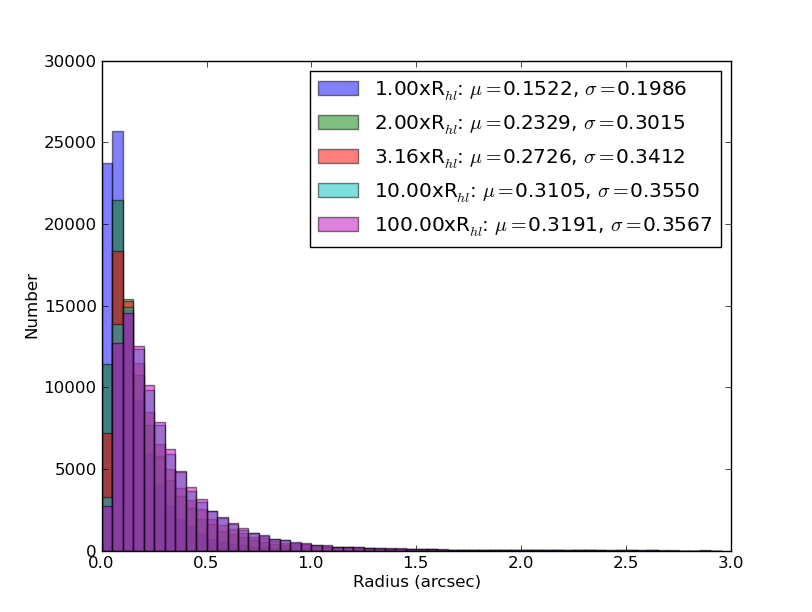
\includegraphics[width=\textwidth]{validation_figures/half_light_hist.png}
\end{subfigure}
\begin{subfigure}[b]{0.4\textwidth}
  \centering
  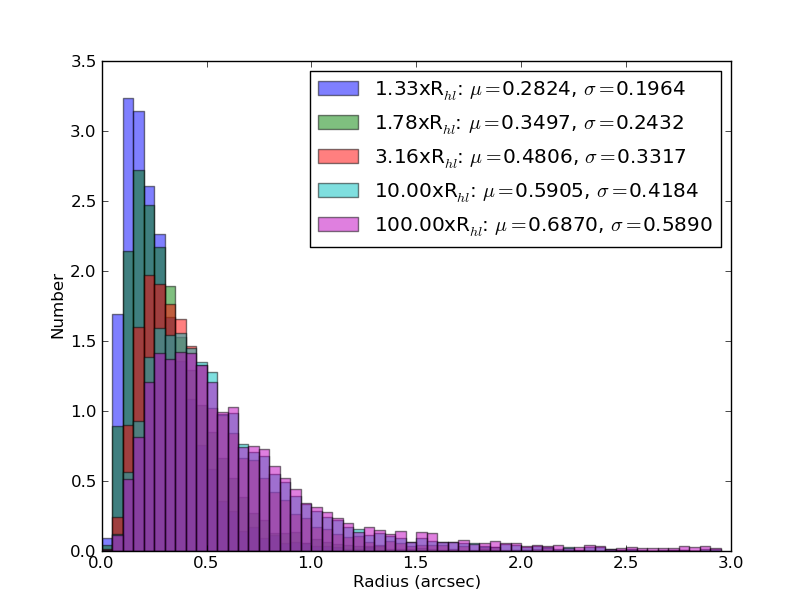
\includegraphics[width=\textwidth]{validation_figures/Second_moment_hist.png}
\end{subfigure}
\caption{Modeling the impact of signal-to-noise on measures of
  radii. The truncation for each distribution is listed in the legend
  along with the mean and standard deviation at that value of the
  truncation.  Truncating the Sersi{\'c} at smaller radii approximates
  lower signal-to-noise measurements.  The left panel shows the
  distributions for half light radii and the right panel for second
  moment radii}
\label{fig:size_hist}
\end{figure}


\begin{figure}[h]
\centering
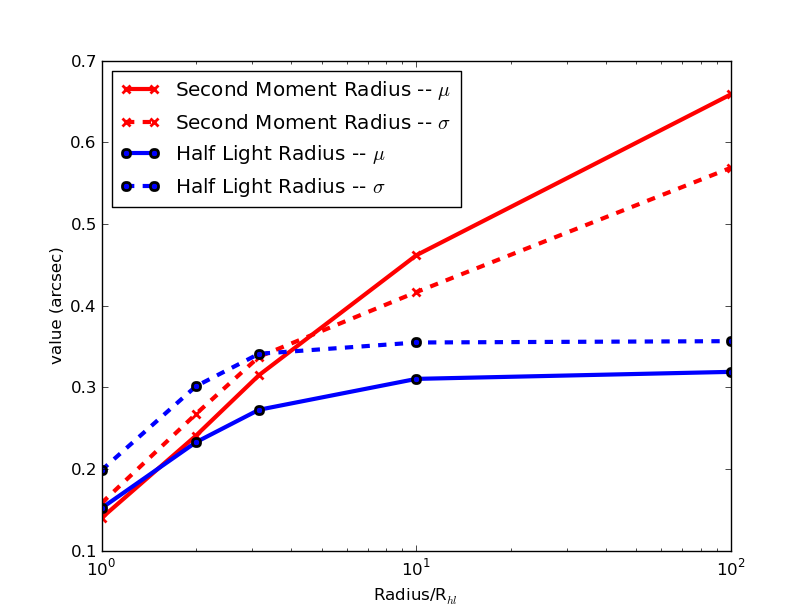
\includegraphics[width=0.5\textwidth]{validation_figures/sec_mom_half_light_mean_sigma.png}
\caption{The mean and standard deviation of the half-light and second
 moment radii as a function of the truncation in the Sersi{\'c} profile.}
\label{fig:mom_hl_line}
\end{figure}

To evaluate the sensitivity of $n_{eff}$ on size, we model the 
half light distribution as a log-normal distribution.  Figure
\ref{fig:ln_fit} shows log-normal fits to the base catalog and COSMOS
data half light radius distributions.  The half light radius
distribution for the base catalog is dominated by the disk components
since there are many more disk-only objects than bulge-only objects
and the disk components have large half light radius values (relative
to the bulge). We measure $n_{eff}$ for a variety of half light radii
distributions by taking the base catalog bulge size distribution and
modeling the disk size distribution as a log-normal distribution.  We
then vary the peak location and width of the disk size distribution
to map the sensitivity of the measure value of $n_{eff}$ to the peak
location and distribution width.
\begin{figure}[h]
\centering
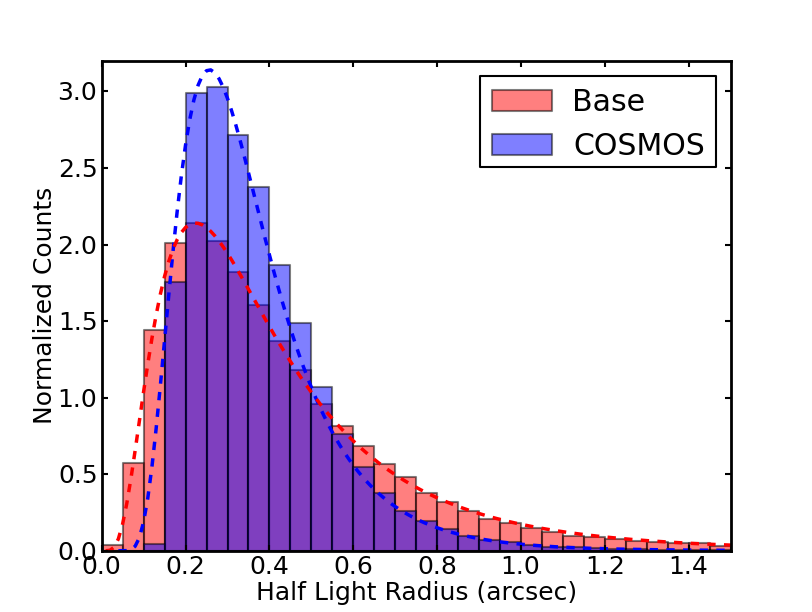
\includegraphics[width=0.5\textwidth]{validation_figures/ln_fit.png}
\caption{The half light radius distributions from the base catalog and 
COSMOS catalog are well fit by a log-normal distribution.  The distributions
are not identical.  Figure \ref{fig:size_sens} shows the impact on the  
measured $n_{eff}$ that having different distributions makes.
    \label{fig:ln_fit}}
\end{figure}

Figure \ref{fig:size_sens} shows the sensitivity of $n_{eff}$ to the
size distribution.  The contours represent the change in $n_{eff}$
(from its nominal value) as a function of distribution width and
peak. Over-plotted are points corresponding to the best fit log-normal
distributions to the COSMOS data set (black circle) and the base
catalog data set (black square).  The difference between the COSMOS
distribution and the base catalog size distributions results in a
change in $n_{eff}$ of less than two.

Combining in quadrature the error in $n_{eff}$ from the shape noise of
the galaxies, the size distributions of the galaxies, and the
signal-to-noise of the observations the total $n_{eff}$ uncertainty is
$1.8$, which meets the requirement of $\pm6$ specified for {\it
  Catalogs: Requirement 3}


\begin{figure}[h]
\centering
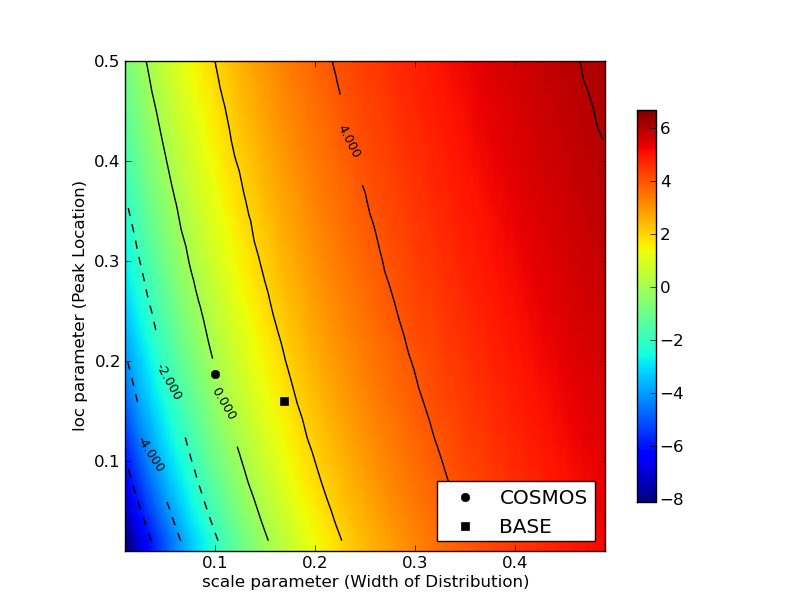
\includegraphics[width=0.5\textwidth]{validation_figures/size_sensitivity.png}
\caption{Sensitivity of the predicted $n_{eff}$ to the shape of the
  half light radius distribution.  The surface is normalized to the
  value of $n_{eff}$ as measured using the half light radius
  distribution from COSMOS.  The black circle is the location of the
  COSMOS data (which by construction falls on the zero contour).  The
  black square is the prediction of the measured $n_{eff}$ using the
  half light radius distribution from the base
  catalog.\label{fig:size_sens}}
\end{figure}

\subsection{Catalogs: Requirement 4}

{\it Photometric performance: For the photometric calibration
  simulations the distribution of stellar colors shall encompass the
  colors of white dwarfs through red giant branch stars.  The median
  color distributions of stars must trace the observed color locus for
  these stars to within the 0.02 magnitudes (averaged over intervals
  of 0.3 magnitudes in color). These requirements are defined for
  Galactic latitudes $|b|>30$.}\\


In order to evaluate the sensitivity of the photometric calibration to
the distributions of stars within a focal plane, the Galactic model
must have realistic color distributions.  This includes both the range
of colors spanned by the stellar sources and the fidelity to which
these stars reproduce the observed stellar locus. In Figure
\ref{fig:starcolorspan} we verify that the stellar catalog meets the
requirement that the colors span the range given in {\it Catalogs:
  requirement 4},
\begin{center}
\begin{tabular}{c|r|r}
  Color Range& Blue Density (deg$^{-2}$) & Red Density (deg$^{-2}$)\\
\hline
  $ -0.2 < u-g <        2.7 $&9&7\\
  $  -0.4  <  g-r <       1.7 $&18&200\\
  $ -0.3   <  r-i <    2.3 $&23&44\\
  $  -0.25 < i-z <       1.2 $&255&42\\ 
  $  -0.2 <  z-y   <    0.8 $&967&6
\end{tabular}
\end{center}
For each color ($u-g$, $g-r$, $r-i$, $i-z$, and $z-y$) we plot the
normalized histogram for the main sequence and red giant branch (RGB)
stars (forward hatching) and the white dwarf (backward hatching).
Together the two distributions span the required range as shown by the
dashed vertical lines in each panel (the density of stars at the blue
and red extrema of these distributions is noted in the table above). 
\begin{figure}[h]
\centering
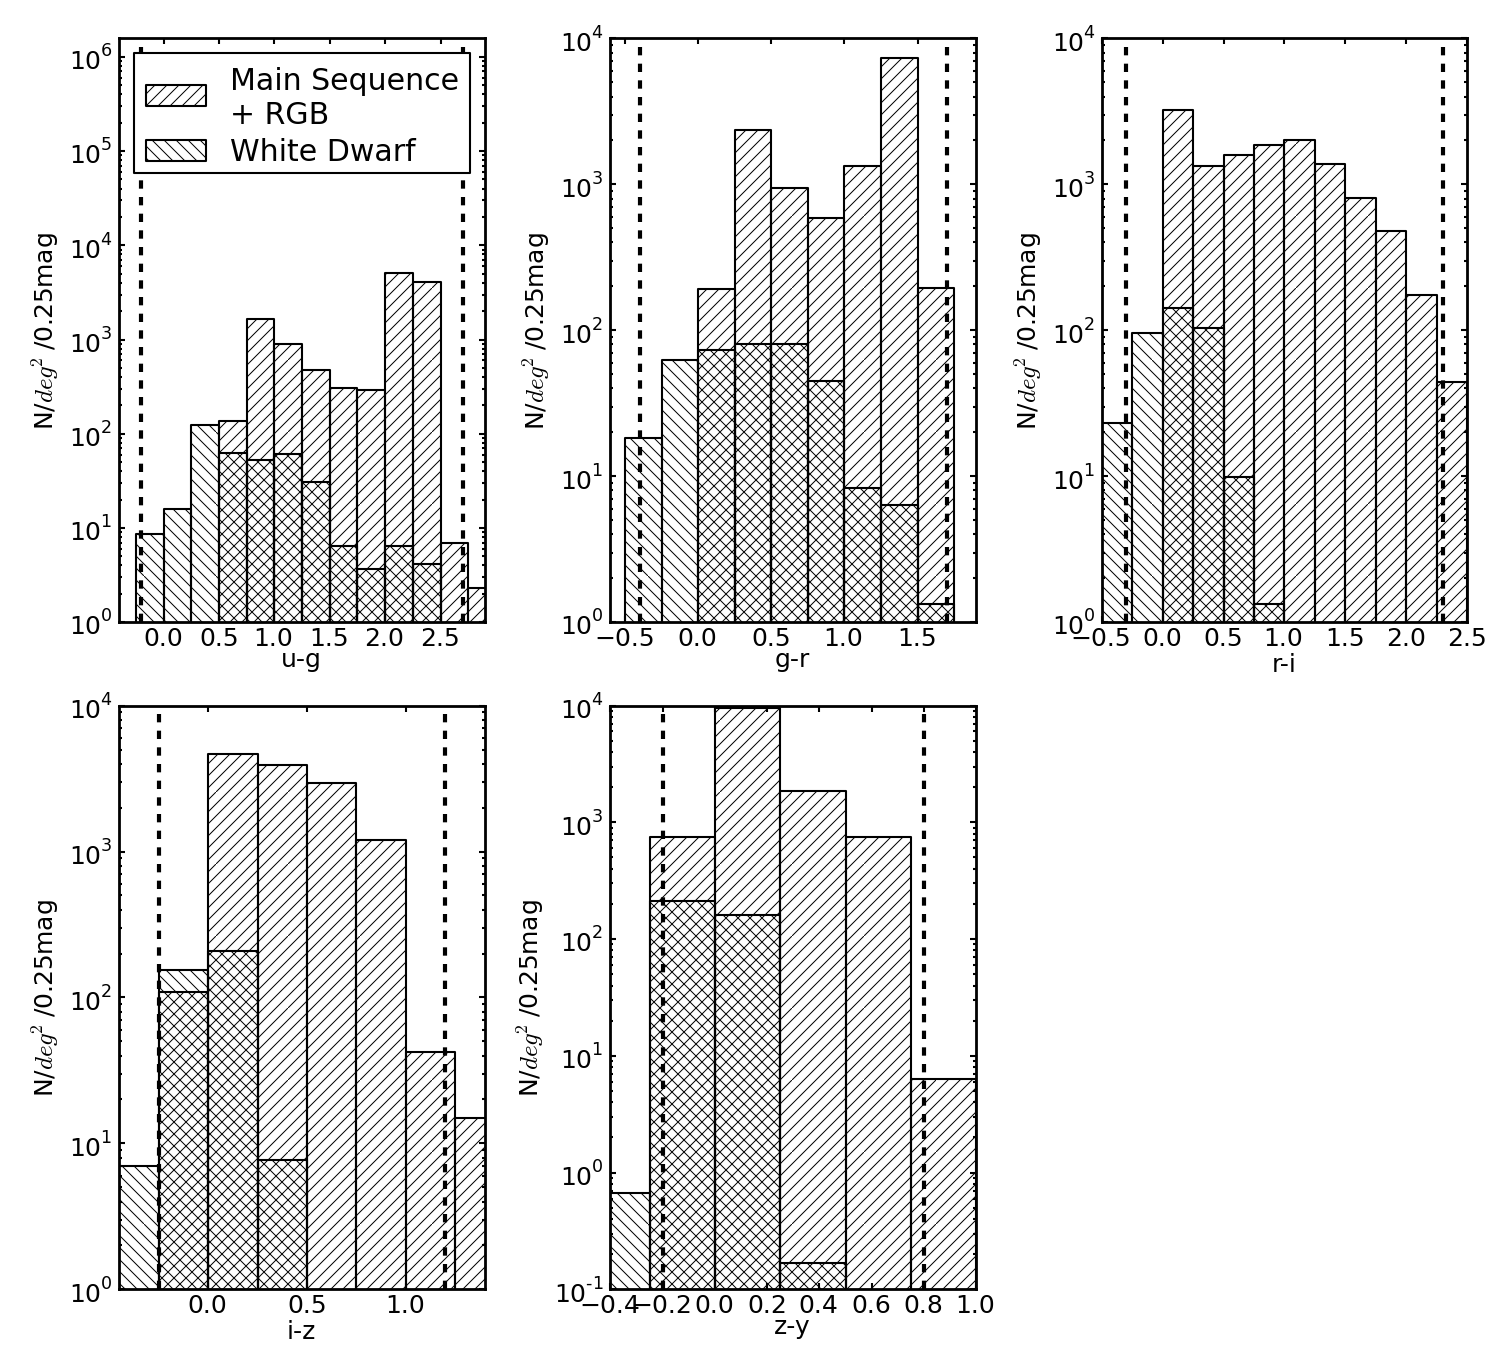
\includegraphics[width=0.5\textwidth]{validation_figures/star_lsst_color_hist.png}
\caption{Normalized counts of main sequence, red giant branch and white dwarf stars as a function of color.  Heavy dashed lines show the requirements given in the requirements document.\label{fig:starcolorspan}}
\end{figure}

To verify the veracity of the main sequence stellar locus, we use the
principal colors of the stellar locus as described by \citet{helmi02},
and fit for in the SDSS photometric system by \citet{ivezic04}.  We
use stars selected from the same fields as used in the number counts
analysis for all fields with $b<-30$.  In order to avoid complications
associated with the difference between the LSST and SDSS photometric
systems, we calculate the un-extincted magnitudes in the SDSS
bandpasses using the best fit spectrum for each star.  We then
calculate the principal colors for each star using the relations in
\citet{ivezic04}.  \citet{ivezic04} noticed that when fitting for the
coefficents of $P_{2}$ that a magnitude dependent offset remained.
They attributed this to measurement systematics and applied an
empirical correction to the fits in order to remove the $r$ band
dependence of the principal colors.  Since we calculate the photometry
with idealized spectra and throughput curves, we do not notice a trend
with magnitude, and therefore have not applied the empirical
correction used in \citet{ivezic04}.  Figure
\ref{fig:principalcolorshist} shows that the principal colors, as
calculated from the base catalog, are in good agreement with the
location of the stellar locus for the SDSS.  We note that the increase
in scatter in the s band when compared to other colors arises from a
metallicity dependence in the color.  Figure \ref{fig:sfeh} shows this
dependence which is consistent with SDSS observations. The base
catalog meets the $\pm0.02mag$ requirement on the deviation from the
stellar locus to single epoch depth in all 4 principal colors:
${\Delta}s=-0.003, {\Delta}w=0.001, {\Delta}x=-0.005,
{\Delta}y=-0.013$.

\begin{figure}[h]
\centering
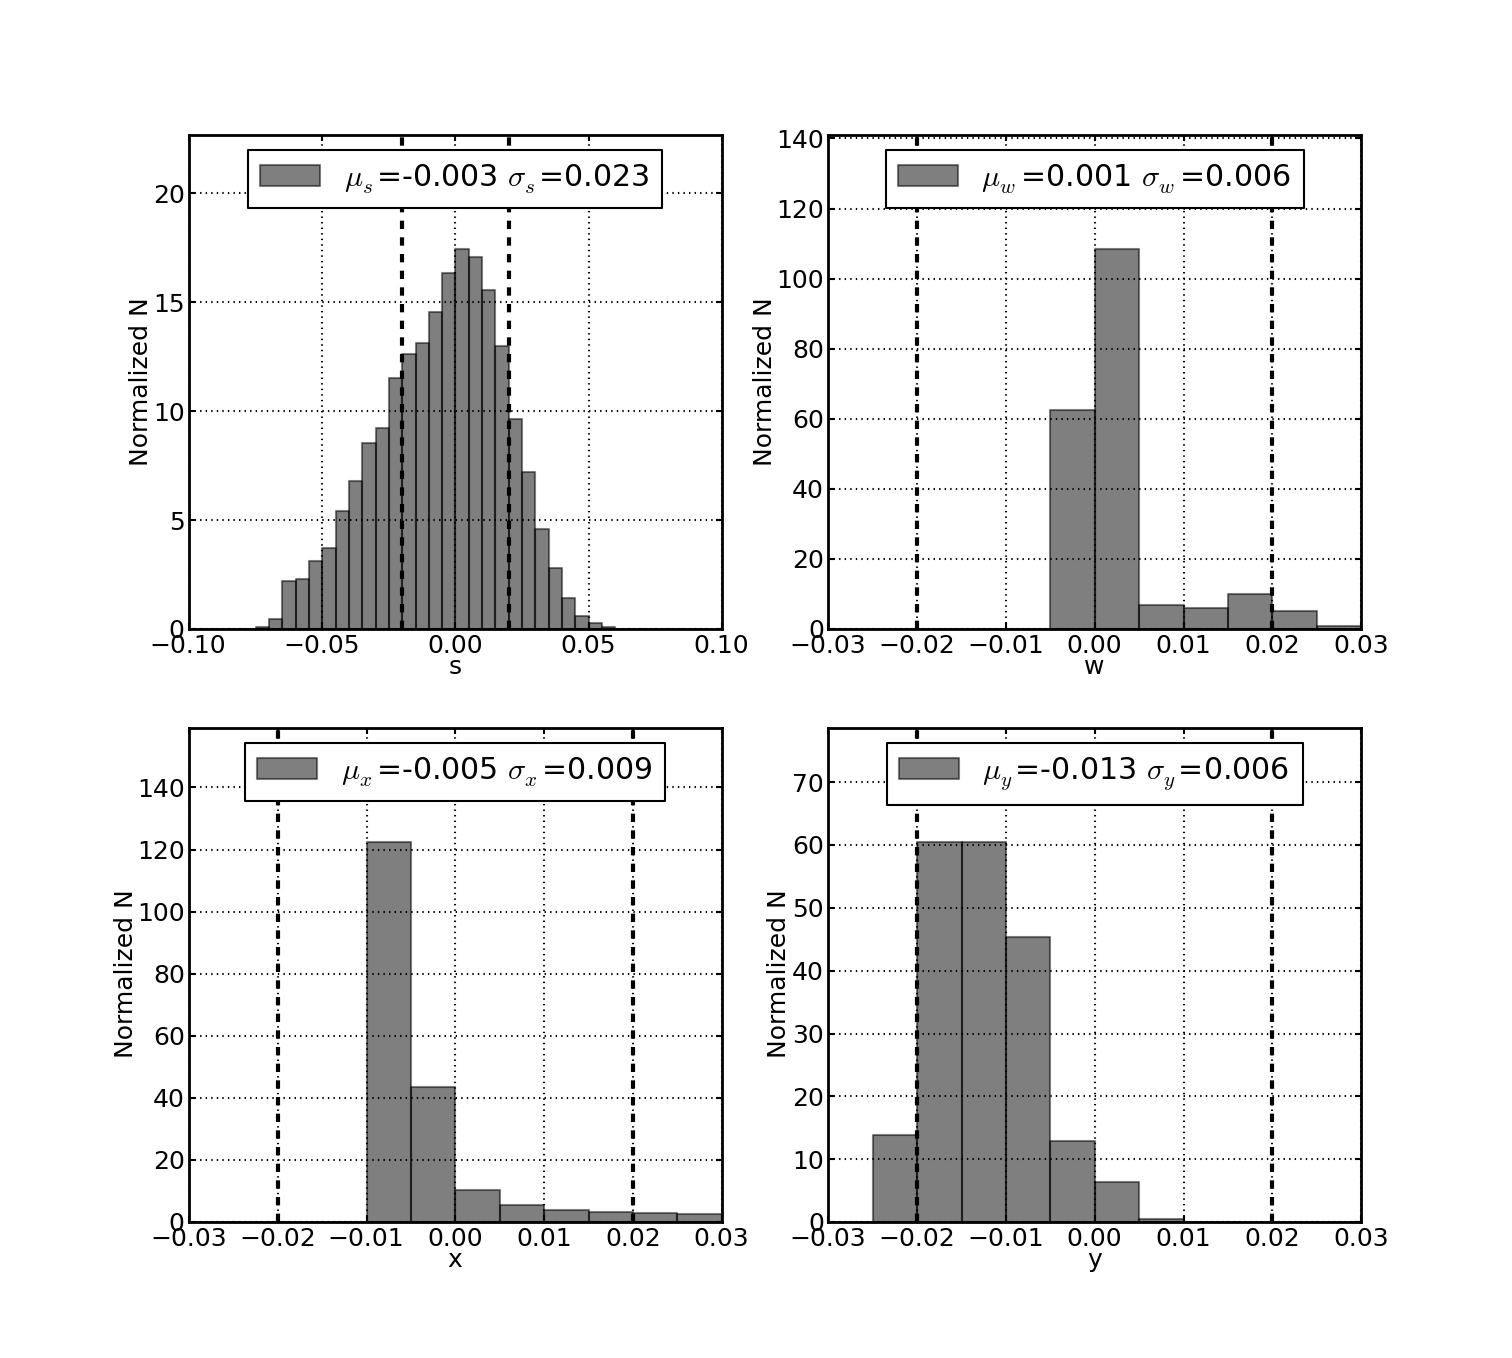
\includegraphics[width=0.5\textwidth]{validation_figures/principal_colors_hist.png}
\caption{Histograms of the principal colors of stars in the base
  catalog compared to SDSS principal colors (zero color in these
  plots) to the stretch single epoch depth of $r < 24.8$. The mean and
  standard deviation for each histogram are given in the legend in the
  upper right.\label{fig:principalcolorshist}}
\end{figure}

\begin{figure} [h]
\centering
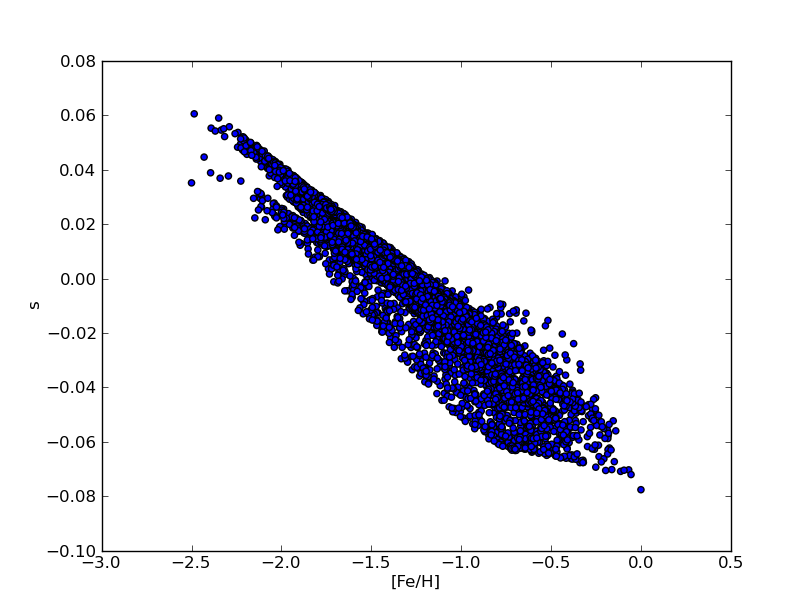
\includegraphics[width=0.5\textwidth]{validation_figures/s_met.png}
\caption{The principal color s as a function of metallicity.\label{fig:sfeh}}
\end{figure}


\subsection{Catalogs Requirement 5}

{\it All models for the astrometric transforms applied to the catalogs
  (including interpolation functions) shall have an rms uncertainty less than 1 mas}\\

All operations on positions are undertaken using double precision
accuracy. Angular operations are converted to Cartesian coordinates to
ensure accuracy at the celestial poles and to minimize the
complications of the coordinate wraparound at the
meridian. Astrometric accuracy of the CatSim simulation framework is
determined from the performance of the Starlink positional astronomy
library (SLALIB; \citealt{wallace}). This software library enables
astrometric transformations and operations with accuracies of the
order of a milliarcsecond or better.  The principal SLALIB routines
used by the CatSim framework are those for precession, nutation,
stellar aberration, rotation of the Earth, diurnal aberration, and
refraction.  As described in \citet{wallace} the definition of ICRS
coordinate system used in SLALIB and its transform to an FK5 (Fifth
Fundamental Catalog - The Basic Fundamental Stars) system has an rms
accuracy that is sub-milliarcsecond. Precession and nutation are based
on the model of \citet{SF2001} and have an rms uncertainty of $<$1
milliarcsecond (with the uncertainty growing at approximately 0.3
milliarcseconds per 1000 years). Aberration and light deflection
corrections are undertaken in an iterative manner with uncertainties
of $<$1 milliarcsecond and the Earth position and velocity corrections
are based on the methods of \citep{stumpff} with a maximum error of
0.3 milliarcseconds. All of these components, added in quadrature, are
consistent with the requirements described in the simulation
requirements document \citet{requirements}.

The largest of the uncertainties in any of the astrometric transforms
are those that arise due to the color dependence of refraction. For a
nominal set of atmospheric conditions (i.e.\ temperature, pressure,
humidity, and lapse rate) the rms astrometric uncertainty is 2.5 mas
over the wavelength range from 0.3 to 1 $\mu$m . This represents a
systematic error on wavelength dependent positions (i.e.\ it is
effectively an error on the parameterization of the model), which is
fit for when deriving an astrometric solution. For the case of CatSim,
while differential chromatic refraction can be applied to catalogs
that are output for science evaluation, the data input to the photon
simulator does not include this effect (i.e.\ it is generated
internally to the photon simulator).

\subsection{Catalogs: Requirement 6}

{\it The system shall be capable of incorporating new astrophysical catalogs without requiring
a redesign of the class-schema framework}\\

The ability to create new catalogs is available within the framework
through the use of user-designed subclasses and class mixins
\citep{mixin}.  New types of catalog can be generated by creating a
new class from the InstanceCatalog base class. Data (i.e.\ output
columns) required by this catalog are defined as class
attributes. These data are then gathered either from the database
directly or using functions methods defined in the class itself. These
data gathering methods can take the form of a {\tt
  get\_[column\_name]} method or in the form of compound columns with
their own {\tt get\_} methods.

The InstanceCatalog metaclass verifies that all new columns specified
for a new catalog or object reside in the database or that they can be
generated by user defined methods and functions.  If no method exists
and there is no associated database entry for the column then an error
is raised. Furthermore, this error is raised prior to the query being
run because the instantiation of the class initiates a dry run of the
table output. As a result, the user is protected from errors prior to
generating the data since all of the necessary columns are determined
during the dry run.

An example of the extension of this class structure is provided
below. For this case the user defines the attributes that they wish to
extract form the database (by creating the {\it BasicCatalog} class)
and the operations they wish to apply to these attributes (by creating
the Python Mixin ({\it AstrometryMixin}). A new catalog type is then
created by combining these classes ({\it CustomCatalog}) that
expresses how to output the data. All of the functions and methods
present within the CatSim framework (including photometric, and
astrometric operations) are available to the new class through this
subclassing process (i.e.\ the user simply defines the new operations
that they need).

This process simplifies the creation of new object types, tables,
functionality, and databases by an external user. 

\begin{verbatim}
class BasicCatalog(InstanceCatalog):
    """Simple catalog with columns directly from the database"""
    catalog_type = 'basic_catalog'
    refIdCol = 'id'
    column_outputs = ['id', 'ra_J2000', 'dec_J2000']
    # transformations specify conversions when moving from the database
    # to the catalog.  In this case, we take RA/DEC in radians and convert
    # to degrees.
    transformations = {"ra_J2000":np.degrees,
                       "dec_J2000":np.degrees}

class AstrometryMixin(object):
    @compound('ra_corrected', 'dec_corrected')
    def get_points_corrected(self):
        ra_J2000 = self.column_by_name('ra_J2000')
        dec_J2000 = self.column_by_name('dec_J2000')
        # ... do the conversions: these are just standins
        ra_corrected = ra_J2000 + 0.001
        dec_corrected = dec_J2000 - 0.001
        return ra_corrected, dec_corrected

class CustomCatalog(BasicCatalog, AstrometryMixin):
    catalog_type = 'custom_catalog'
    refIdCol = 'id'
    column_outputs = ['id', 'redshift', 'points_corrected']
    transformations = {"ra_corrected":np.degrees,
                       "dec_corrected":np.degrees}

# Now to create a catalog, we connect to a database and call write_catalog
db = GalaxyObj()
catalog = CustomCatalog(db)
catalog.write_catalog("out.txt")

# out.txt has the following columns:
# id redshift ra_corrected dec_corrected
\end{verbatim}


\section{Future work}
We have shown that the catalogs framework, as it stands, meets all but
one of the requirements stated in \citet{requirements}.  Future work
is necessary to improve the validity, fidelity, generality, and
breadth of the existing framework and, in particular, to meet the
flow down requirements of individual subsystems.

The future work of the catalog framework will focus on three main
areas: continued validation and quantification of risk (high
priority), engineering development (medium to high priority), and
development for broader scientific assessment (low to medium
priority). These priorities are driven by the LSST project requirements
together with the needs of the science community (with the expectation
that the resources for many of the science assessment tasks will come
from outside of the LSST project).
%{\bf maybe some words here about why we choose the various priority levels}

\subsection{High priority}
The first and highest priority is the completion of the validation
tasks that address areas of risk associated with the project. Primary
amongst these areas is the use of observational data to extend the
validation of the star counts to deeper magnitudes and lower Galactic
latitudes.  With appropriate data from surveys such as
Pan-STARRS, % \ref{panstarss},
the comparison should be straight forward to complete for brighter
magnitudes ($V<23$).
%Of course, addressing any differences that arise is more complicated,
%but since the project has planned for this risk, quantifying any
%discrepancy between the model and reality is the most important
%activity.

The second high priority activity is to add bright O, B and A type
stars to the Galactic structure database and incorporate binary stars
and variability into the model.  This will include the extension of
the Galfast model to these stellar types and the adoption of
distributions of bright stars based on existing all-sky catalogs
(e.g.\ the $V<18$ samples from the USNO, Monet private communication)
%to fill in the bright (and blue) end of the stellar distribution of
%main sequence stars. 
These stars will impact the number density of stars in the plane of
the Galaxy and will impact how the survey is run in practice.
Specifically, very bright stars introduce data artifacts (bleed
trails, blooming, glints, etc.) that cannot be modeled with the
current data set.  Additionally, the wave front sensors and guiding
sensors can be tested against the real bright star distribution on the
sky. The data to accomplish these tasks is in hand.
% with the future work
%adjust the current distributions to match the observed distributions
%where they meet.

The third high priority task is the ability to input realistic galaxy
morphology into simulated images (to evaluate shape measurements).
The PhoSim has the ability to take a super-sampled galaxy image and
sample from it to produce an LSST observation of the galaxy, but the
catalogs do not have a library of realistic galaxies to feed to the
simulator.  The other aspect of this effort is to simplify the SED
handling by creating a set of principal component SEDs for each of the
object types.  This would reduce the overall size of the SED library
and make it possible to simulate a galaxy with an SED per pixel so
that realistic color gradients can be included.

The last high priority activity is to validate the Solar System model
against observed data (i.e.\ to validate the density of asteroids as a
function of limiting magnitude).  Since Solar System surveys are
typically either shallow or cover a limited area, and focus at
opposition, a full validation of the Solar System model has been
difficult to achieve.  The Pan-STARRS survey has been running for
three years and will soon have enough data to put constraints on how
well the \citet{grav11} model represents our Solar System (for
$V<21.5$).


\subsection{Medium Priority}


Realistic galaxy morphology will expose failure modes in the
algorithms that do not exist with simplistic and symmetric galaxy
models, but if there is no gravitational shear in the catalog there is
no signal to compare to the noise introduced by this complexity.  The
catalogs framework is capable of handling a per galaxy weak lensing
shear parametrization.  Working with the Science Collaborations the
galaxy catalogs will be extended to incorporate gravitational shear maps
to the galaxy catalogs so that the shear correlation is consistent
with the galaxy large-scale structure.

The ability to simulate realistic errors at the catalogs level
(without having to go through image simulation and measurement) is a
functionality that is required by multiple groups.  This includes,
photometric and astrometric calibration, engineering tests to evaluate
the distributions of bright stars for ghosts and glints, and guide and
wavefront stars. This requires the implementation of an error model
for the LSST that is dependent on seeing, airmass, sky brightness, and
a geometric model for the parameterization of the LSST focal plane
(i.e.\ to define where stars will fall on sensors).


\subsection{Lower Priority}

The lower priority tasks are upgrades to the framework and mostly
facilitate scientific capability analysis.  The first of these is the
implementation of variability that utilizes a higher fidelity
variability model.  Supernovae, for example, have a spectro-temporal
surface that defines the SED of the supernova at any instant in time
given a set of parameters.  This means that an SED per observation
must be produced.  This sort of variability could also be used by the
RR Ly variability model and potentially the AGN variability model.

There is no global supernova model in the base catalogs framework.
Over the lifetime of the survey, there will be approximately one
billion supernovae in the full survey volume.  Significant effort must
be put into making any supernova model deterministic and fast.  The
supernovae must be distributed realistically with respect to the
galaxy distribution.  It is expected that these tools will be provided
by the science collaborations but will require integrating into the
simulation framework.

Further functionality development will be required to support the
integration of external user catalogs and databases. These will
include wide area cosmological models, and science targeted catalogs
(e.g.\ extended and high density sources in the Galaxy, strong
lensing, low surface brightness galaxies, high proper motion stars).
As with the supernovae model, many of these catalogs will be provided
by external users but will require support and documentation from the
CatSim team.


\bibliographystyle{plainnat}
\bibliography{validation}
\end{document}
